\documentclass{article}

% TODO, for submission
% - Remove [preprint]
% - Remove title footnote
% - Add checklist
% - Remove vspace in Section 2 Heading

% if you need to pass options to natbib, use, e.g.:
%     \PassOptionsToPackage{numbers, compress}{natbib}
% before loading neurips_2024


% ready for submission
%\usepackage{neurips_2024}
%\usepackage[preprint]{neurips_2024}
\usepackage[final]{neurips_2024}

% to compile a preprint version, e.g., for submission to arXiv, add add the [preprint] option
% to compile a camera-ready version, add the [final] option
% to avoid loading the natbib package, add option nonatbib:
%    \usepackage[nonatbib]{neurips_2024}

\usepackage[utf8]{inputenc} % allow utf-8 input
\usepackage[T1]{fontenc}    % use 8-bit T1 fonts
\usepackage{hyperref}       % hyperlinks
\usepackage{url}            % simple URL typesetting
\usepackage{booktabs}       % professional-quality tables
\usepackage{amsfonts}       % blackboard math symbols
\usepackage{nicefrac}       % compact symbols for 1/2, etc.
\usepackage{microtype}      % microtypography
\usepackage{xcolor}         % colors

%%%%%%%%%%%%%%%%%%%%%%%%%%%%%%%%%%%%%
% WE ADD HERE ADDITIONAL PACKAGES
%%%%%%%%%%%%%%%%%%%%%%%%%%%%%%%%%%%%%
\usepackage{mathtools}
\usepackage{subcaption}
\usepackage{wrapfig}
\usepackage{cite}           % magical 
\usepackage[ruled, vlined]{algorithm2e}
\usepackage{sidecap}
\usepackage{array}
\sidecaptionvpos{figure}{c}
% Tikz
\usepackage{tikz}
\usetikzlibrary{arrows,arrows.meta,calc}
\usetikzlibrary{patterns,backgrounds}
\usetikzlibrary{positioning,fit}
\usetikzlibrary{shapes.geometric,shapes.multipart}
\usetikzlibrary{patterns.meta,decorations.pathreplacing,calligraphy}
\usetikzlibrary{tikzmark}
\usetikzlibrary{decorations.pathmorphing}

%%%%%%%%%%%%%%%%%%%%%%%%%%%%%%%%%%%%%
% COMMANDS
%%%%%%%%%%%%%%%%%%%%%%%%%%%%%%%%%%%%%
\newcommand{\x}{\mathbf{x}}
\newcommand{\z}{\mathbf{z}}
\newcommand{\y}{\mathbf{y}}
\newcommand{\w}{\mathbf{w}}
\newcommand{\bo}{\mathbf{o}}
\newcommand{\ba}{\mathbf{a}}
\newcommand{\bz}{\mathbf{z}}
\newcommand{\bs}{\mathbf{s}}
\newcommand{\scoref}{\nabla_\x \log p^\tau(\x)}
\newcommand{\scorem}{\mathbf{S}_\theta(\x, \tau)}
\newcommand{\bbe}{\mathbb{E}}
\newcommand{\Tau}{\mathcal{T}}

\newcommand{\repolink}{\href{https://github.com/eloialonso/diamond}{\texttt{https://github.com/eloialonso/diamond}}}
\newcommand{\wslink}{\href{https://diamond-wm.github.io}{\texttt{https://diamond-wm.github.io}}}
%\newcommand{\repolink}{\href{https://anonymous.4open.science/r/_diamond}{\textit{https://anonymous.4open.science/r/\_diamond}}}


\title{Diffusion for World Modeling:\\Visual Details Matter in Atari\thanks{To prevent confusion, this is the final version of \citep{alonso2023diffusion} and is not related to \citep{ding2024diffusion}.}}


% The \author macro works with any number of authors. There are two commands
% used to separate the names and addresses of multiple authors: \And and \AND.
%
% Using \And between authors leaves it to LaTeX to determine where to break the
% lines. Using \AND forces a line break at that point. So, if LaTeX puts 3 of 4
% authors names on the first line, and the last on the second line, try using
% \AND instead of \And before the third author name.

\author{%
  Eloi Alonso\thanks{Equal contribution. $^\ddagger$Equal supervision. Contact: \texttt{eloi.alonso@unige.ch} and \texttt{adam.jelley@ed.ac.uk}}\\
  University of Geneva
  \And
  Adam Jelley$^*$\\ 
  University of Edinburgh
  \And
  Vincent Micheli\\
  University of Geneva
  \And
  Anssi Kanervisto\\
  Microsoft Research
  \And
  Amos Storkey\\
  University of Edinburgh
  \And
  Tim Pearce$^\ddagger$\\\
  Microsoft Research
  \And
  Fran\c{c}ois Fleuret$^\ddagger$\\
  University of Geneva
}
% \author{%
%   David S.~Hippocampus\thanks{Use footnote for providing further information
%     about author (webpage, alternative address)---\emph{not} for acknowledging
%     funding agencies.} \\
%   Department of Computer Science\\
%   Cranberry-Lemon University\\
%   Pittsburgh, PA 15213 \\
%   \texttt{hippo@cs.cranberry-lemon.edu} \\
  % examples of more authors
  % \And
  % Coauthor \\
  % Affiliation \\
  % Address \\
  % \texttt{email} \\
  % \AND
  % Coauthor \\
  % Affiliation \\
  % Address \\
  % \texttt{email} \\
  % \And
  % Coauthor \\
  % Affiliation \\
  % Address \\
  % \texttt{email} \\
  % \And
  % Coauthor \\
  % Affiliation \\
  % Address \\
  % \texttt{email} \\
% }




\begin{document}


\maketitle


\begin{abstract}
Segment Anything Model 2 (SAM 2) has emerged as a powerful tool for video object segmentation and tracking anything. Key components of SAM 2 that drive the impressive video object segmentation performance include a large multistage image encoder for frame feature extraction and a memory mechanism that stores memory contexts from past frames to help current frame segmentation. The high computation complexity of multistage image encoder and memory module has limited its applications in real-world tasks, e.g., video object segmentation on mobile devices. To address this limitation, we propose EfficientTAMs, lightweight track anything models that produce high-quality results with low latency and model size. Our idea is based on revisiting the plain, nonhierarchical Vision Transformer (ViT) as an image encoder for video object segmentation, and introducing an efficient memory module, which reduces the complexity for both frame feature extraction and memory computation for current frame segmentation. We take vanilla lightweight ViTs and efficient memory module to build EfficientTAMs, and train the models on SA-1B and SA-V datasets for video object segmentation and track anything tasks. We evaluate on multiple video segmentation benchmarks including semi-supervised VOS and promptable video segmentation, and find that our proposed EfficientTAM with vanilla ViT perform comparably to SAM 2 model (HieraB+SAM 2) with $\sim$2x speedup on A100 and $\sim$2.4x  parameter reduction. On segment anything image tasks, our EfficientTAMs also perform favorably over original SAM with $\sim$20x  speedup on A100 and $\sim$20x  parameter reduction. On mobile devices such as iPhone 15 Pro Max, our EfficientTAMs can run at $\sim$10 FPS for performing video object segmentation with reasonable quality, highlighting the capability of small models for on-device video object segmentation applications. 
\end{abstract}
\section{Introduction}
Reinforcement Learning from Human Feedback (RLHF) is a technique that can be used to align an agent --- such as a Large Language Model (LLM) --- to human preferences and lead to more truthful, more helpful, less harmful and more preferred outputs \cite{ouyang2022training}. Proximal Policy Optimization (PPO) \cite{schulman2017proximal} and Direct Preference Optimization (DPO) \cite{rafailov2023direct} are two such aligment techniques which have been extensively used to improve the quality of LLM outputs, leading to instruction following agents or chat assistants which are quickly approaching human-baselines in a variety of knowledge and reasoning tasks \cite{open-llm-leaderboard, clark2018think, zellers2019hellaswag, hendrycks2021measuring, lin2022truthfulqa, DBLP:journals/corr/abs-1907-10641, DBLP:journals/corr/abs-2110-14168}.

However, recent research has shown that RLHF may actually hurt an LLM's reasoning abilities rather than improving it. One study \cite{bekbayev2023poison} discovered that performing alignment during the Supervised Fine-Tuning (SFT) stage of training may lead to worse performance on reasoning benchmarks, and another \cite{bai2022training} discovered that SFT alone outperforms RLHF for smaller models with the benefits of RLHF only emerging for models with more than 1 Billion parameters. Ouyang et al. \cite{ouyang2022training} also reports an increased tendency for RLHF models to make up information in closed domain tasks (``hallucination'') compared to models trained with SFT alone.

To combat the the risk of RLHF compromising the abilities of an LLM in favor of producing preferable outputs we introduce Direct Preference Heads (DPH), a novel feature based approach that optimises a reward score produced by the LLM rather than optimising the logits produced by language modelling head. DPH can be used in combination with (or without) existing alignment techniques to allow language models to self-evaluate outputs sampled at inference time and select the highest scoring candidate.

We evaluate the performance of DPH using an efficient 551M parameter LM on a variety of commonsense reasoning and Natural Language Understanding (NLU) tasks. All code used to train our models is available on \anon{\href{https://github.com/Avelina9X/direct-preference-heads}{GitHub}} and we release our model weights on \anon{\href{https://huggingface.co/collections/Avelina/direct-preference-heads-preprint-6612d8a6fa3843352943fd43}{Hugging Face}}.
\vspace{-0.1cm}
\section{Preliminaries}
\label{sec:framework}
\vspace{-0.1cm}

\subsection{Reinforcement learning and world models}
\label{subsec:pomdp_and_wm}

We model the environment as a standard Partially Observable Markov Decision Process (\textsc{pomdp}) \citep{sutton2018reinforcement}, $(\mathcal{S}, \mathcal{A}, \mathcal{O},T,R,O,\gamma)$, where $\mathcal{S}$ is a set of states, $\mathcal{A}$ is a set of discrete actions, and $\mathcal{O}$ is a set of image observations. The transition function $T: \mathcal{S} \times \mathcal{A} \times \mathcal{S} \to [0,1]$ describes the environment dynamics $p(\mathbf{s}_{t+1} \mid \mathbf{s}_t, \ba_t)$, and the reward function $R: \mathcal{S} \times \mathcal{A} \times \mathcal{S} \to \mathbb{R}$ maps transitions to scalar rewards. Agents cannot directly access states $s_t$ and only see the environment through image observations $x_t \in \mathcal{O}$, emitted according to observation probabilities $p(\x_t \mid \mathbf{s}_t)$, described by the observation function $O: \mathcal{S} \times \mathcal{O} \to [0,1]$. The goal is to obtain a policy $\pi$ that maps observations to actions in order to maximize the expected discounted return $\mathbb{E}_\pi[\sum_{t \ge 0} \gamma^t r_t]$, where $\gamma \in [0,1]$ is a discount factor. World models \citep{ha2018world} are generative models of environments, i.e. models of $p(s_{t+1},r_{t} \mid s_t, a_t)$. These models can be used as simulated environments to train RL agents \citep{sutton1991dyna} in a sample-efficient manner \citep{wu2023daydreamer}. In this paradigm, the training procedure typically consists of cycling through the three following steps: collect data with the RL agent in the real environment; train the world model on all the collected data; train the RL agent in the world model environment (commonly referred to as "in imagination"). 

\subsection{Score-based diffusion models}
\label{subsec:diffusion}

Diffusion models \citep{sohl2015difforigin} are a class of generative models inspired by non-equilibrium thermodynamics that generate samples by reversing a noising process.

We consider a diffusion process $\{\x^\tau\}_{\tau \in [0,\Tau]}$ indexed by a continuous time variable $\tau \in [0,\Tau]$, with corresponding marginals $\{p^\tau\}_{\tau \in [0,\Tau]}$, and boundary conditions $p^0 = p^{data}$ and $p^\Tau = p^{prior}$, where $p^{prior}$ is a tractable unstructured prior distribution, such as a Gaussian. Note that we use $\tau$ and superscript for the diffusion process time, in order to keep $t$ and subscript for the environment time.

This diffusion process can be described as the solution to a standard stochastic differential equation (SDE) \citep{song_sde},
\begin{equation}
\label{eq:forward_process}
    d\x = \mathbf{f} (\x, \tau) d\tau +  g(\tau) d\w, 
\end{equation}
where $\w$ is the Wiener process (Brownian motion), $\mathbf{f}$ a vector-valued function acting as a drift coefficient, and  $g$ a scalar-valued function known as the diffusion coefficient of the process.

To obtain a generative model, which maps from noise to data, we must reverse this process. Remarkably, \citet{anderson1982reverse} shows that the reverse process is also a diffusion process, running backwards in time, and described by the following SDE,
\begin{equation}
\label{eq:reverse_process}
    d\x = [\mathbf{f} (\x, \tau) - g(\tau)^2 \scoref] d\tau +  g(\tau) d\Bar{\w}, 
\end{equation}
where $\Bar{\w}$ is the reverse-time Wiener process, and $\scoref$ is the (Stein) score function, the gradient of the log-marginals with respect to the support. Therefore, to reverse the forward noising process, we are left to define the functions $f$ and $g$ (in Section \ref{subsec:practical_dwm}), and to estimate the unknown score functions $\scoref$, associated with marginals $\{p^\tau\}_{\tau \in [0,\Tau]}$ along the process. In practice, it is possible to use a single time-dependent score model $\scorem$ to estimate these score functions \citep{song_sde}.

At any point in time, estimating the score function is not trivial since we do not have access to the true score function. Fortunately, \citet{hyvarinen2005estimation} introduces the \textit{score matching} objective, which surprisingly enables training a score model from data samples without the knowledge of the underlying score function. To access samples from the marginal $p^\tau$, we need to simulate the forward process from time $0$ to time $\tau$, as we only have clean data samples. This is costly in general, but if $f$ is affine, we can analytically reach any time $\tau$ in the forward process in a single step, by applying a Gaussian perturbation kernel $p^{0\tau}$ to clean data samples \citep{song_sde}. Since the kernel is differentiable, score matching simplifies to a \textit{denoising score matching} objective \citep{vincent2011connection},

\begin{equation}
\label{eq:denoising_sm}
    \mathcal{L}(\theta) = \bbe \left[ \Vert \mathbf{S}_\theta(\x^\tau, \tau) - \nabla_{\x^\tau} \log p^{0\tau}(\x^\tau \mid \x^0) \Vert^2 \right],
\end{equation}

where the expectation is over diffusion time $\tau$, noised sample $\x^\tau \sim p^{0\tau}(\x^\tau \mid \x^0)$, obtained by applying the $\tau$-level perturbation kernel to a clean sample $\x^0 \sim p^{data}(\x^0)$. Importantly, as the kernel $p^{0\tau}$ is a known Gaussian distribution, this objective becomes a simple $L_2$ reconstruction loss,

\begin{equation}
\label{eq:reconstruction_sm}
     \mathcal{L}(\theta) = \bbe \left[ \Vert \mathbf{D}_\theta(\x^\tau, \tau) - \x^{0} \Vert^2 \right],
\end{equation}

with reparameterization $\mathbf{D}_\theta(\x^\tau, \tau) = \mathbf{S}_\theta(\x^\tau, \tau) \sigma^2(\tau) + \x^\tau$, where $\sigma(\tau)$ is the variance of the $\tau$-level perturbation kernel.



\subsection{Diffusion for world modeling}
\label{subsec:dwm_training}

%The score-based diffusion model described in Section \ref{subsec:diffusion} provides an unconditional generative model of $p_{data}$. To serve as a world model, we need a conditional generative model of the environment dynamics, $p(s_{t+1} \mid s_t, a_t)$. Since we consider the more general case of a \textsc{pomdp} where the Markovian state is unknown, we instead approximate this state with a buffer of recent observations and actions. We condition a diffusion model  with this buffer, to estimate $p(\x_{t+1} \mid \x_{\le t}, a_{\le t})$ and generate the next observation directly, as demonstrated in Figure \ref{fig:architecture}. This modifies Equation \ref{eq:reconstruction_sm} as follows,

The score-based diffusion model described in Section \ref{subsec:diffusion} provides an unconditional generative model of $p_{data}$. To serve as a world model, we need a conditional generative model of the environment dynamics, $p(\x_{t+1} \mid \x_{\le t}, a_{\le t})$, where we consider the general case of a \textsc{pomdp}, in which the Markovian state $s_t$ is unknown and can be approximated from past observations and actions. We can condition a diffusion model on this history, to estimate and generate the next observation directly, as shown in Figure \ref{fig:architecture}. This modifies Equation \ref{eq:reconstruction_sm} as follows,
\begin{equation}
\label{eq:denoising_sm_conditional}
     \mathcal{L}(\theta) = \bbe \left[ \Vert \mathbf{D}_\theta(\x_{t+1}^\tau, \tau, \x_{\le t}^0, a_{\le t}) - \x_{t+1}^0 \Vert^2 \right].
\end{equation}
\vspace{-5mm}

During training, we sample a trajectory segment $\x_{\le t}^0, a_{\le t}, \x_{t+1}^0$ from the agent's replay dataset, and we obtain the noised next observation $\x_{t+1}^\tau \sim p^{0\tau}(\x_{t+1}^\tau \mid \x_{t+1}^0)$ by applying the $\tau$-level perturbation kernel. In summary, this diffusion process for world modeling resembles the standard diffusion process described in Section \ref{subsec:diffusion}, with a score model conditioned on past observations and actions.

To sample the next observation, we iteratively solve the reverse SDE in Equation \ref{eq:reverse_process}, as illustrated in Figure \ref{fig:architecture}. While we can in principle resort to any ODE or SDE solver, there is an inherent trade-off between sampling quality and Number of Function Evaluations (NFE), that directly determines the inference cost of the diffusion world model (see Appendix \ref{appendix:sampling} for more details).

\section{Method}
\label{sec:method}

\begin{figure*}[t]
    \centering
    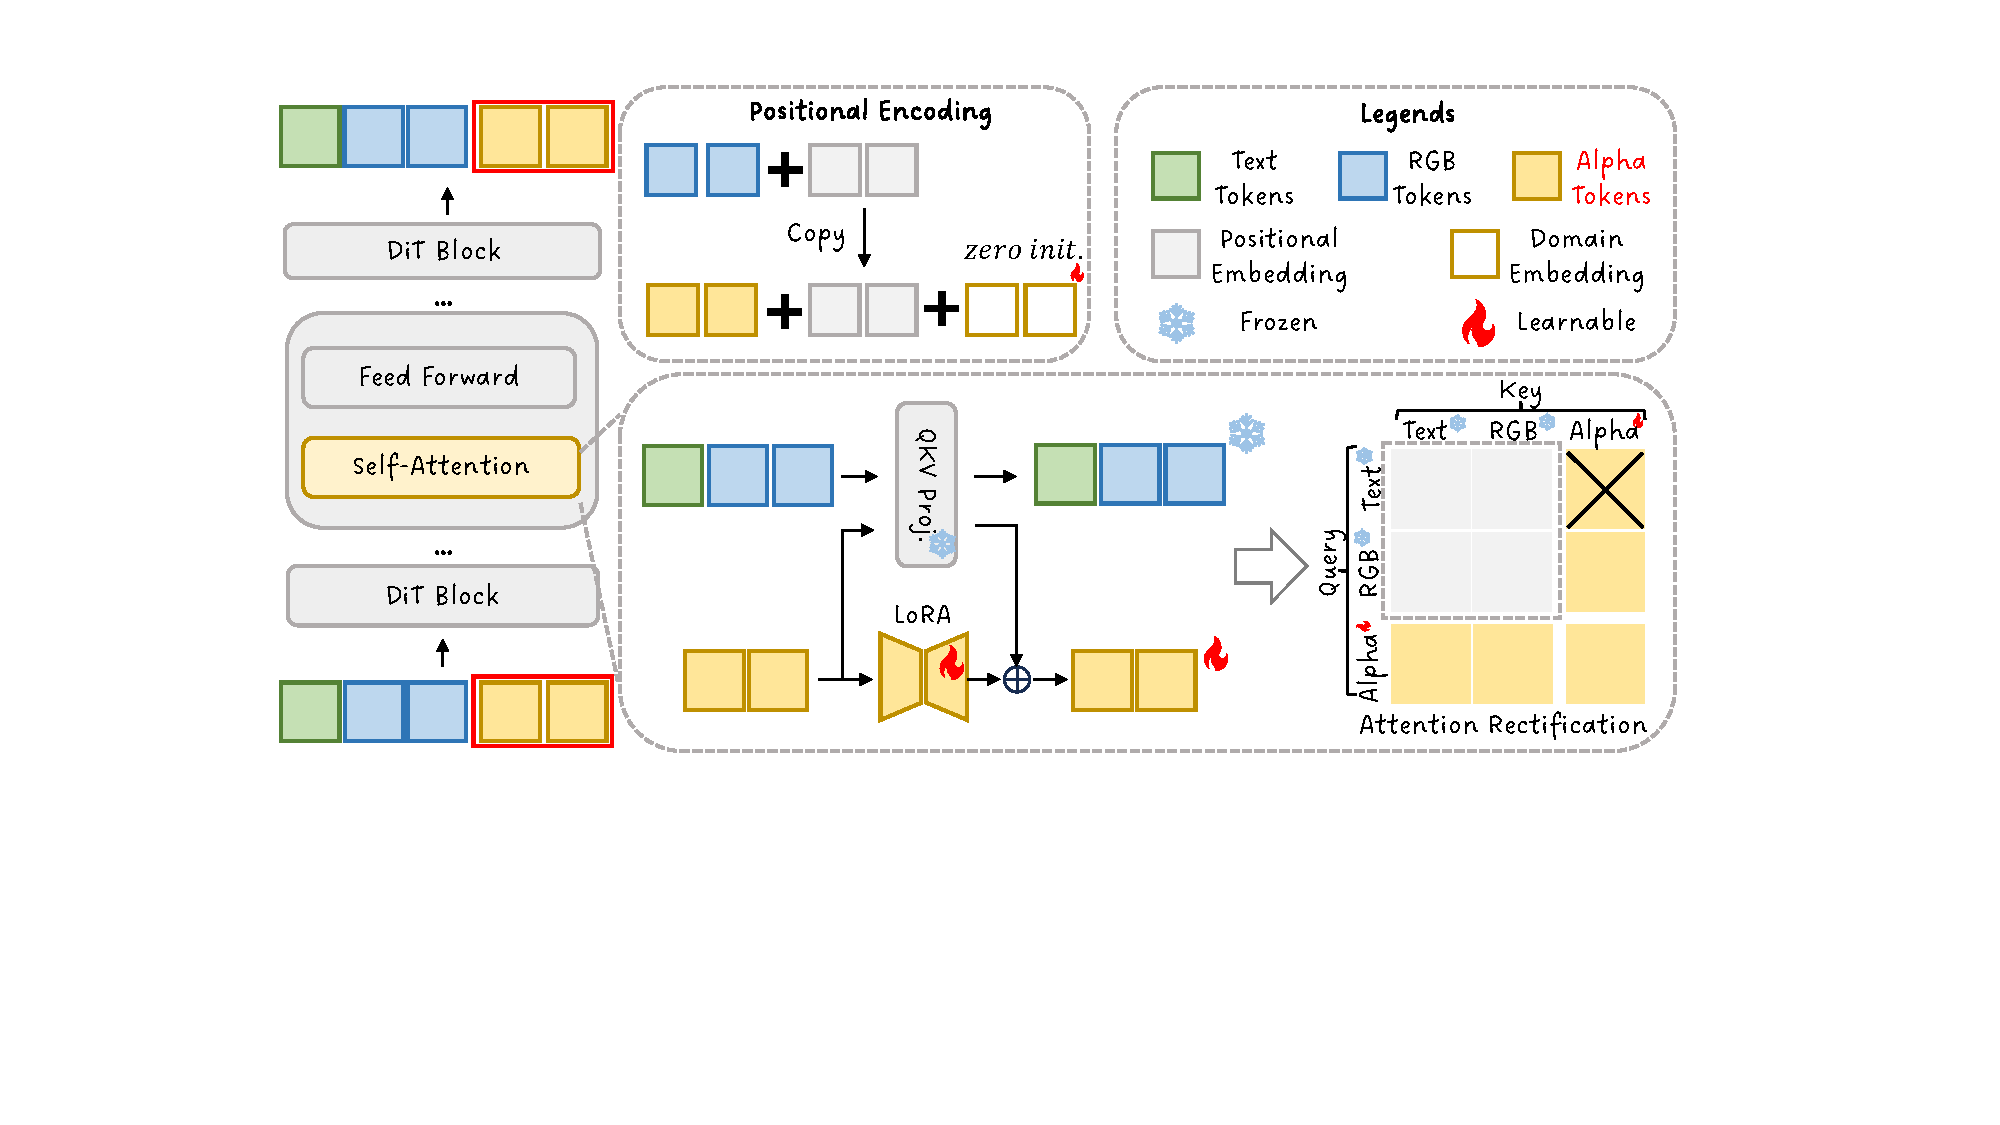
\includegraphics[width=1.0\linewidth]{figs/method-pipeline.pdf}
    \vspace{-0.2in}
    \caption{\textbf{Pipeline of TransPixar.} Our method is organized as follows: (1) \textbf{Left}: we extend the input of DiT to include new alpha tokens; (2) \textbf{Top Center}: we initialize alpha tokens with our positional encoding; (3) \textbf{Bottom Cente}r: we insert a partial LoRA and adjust attention computation during training and inference.}
    \label{fig-pipeline}
    \vspace{-0.1in}
\end{figure*}


% %-------------------------------------------------------------------------
\subsection{Preliminary}
We first introduce the open-sourced state-of-the-art DiT-based video generation models~\cite{yang2024cogvideox,genmo2024mochi}.
The core components of DiT-based video models are attention modules, and there are two primary distinctions between these models and previous approaches.
On one hand, unlike previous models that alternate between 1D temporal attention and 2D spatial attention~\cite{cerspense2023zeroscope, chen2023videocrafter1, chen2024videocrafter2, opensora}, current methods typically employ 3D spatio-temporal attention, allowing them to capture spatio-temporal dependencies more effectively.
On the other hand, instead of using cross-attention for text conditioning, these models concatenate text tokens \( \mathbf{x}_{\text{text}} \) with visual tokens \( \mathbf{x}_{\text{video}} \) into a single long sequence. 
The shape of video tokens and text tokens are \(B\times L\times D\) and \(B\times L_{\text{text}}\times D\), wher \(B\) equals to batch size, \(L_{\text{text}}\) equals to the length of text tokens, \(L\) equals to the length of video tokens and \(D\) equals to the latent dimension of transformer.
Full self-attention is then applied across the combined sequence:
\begin{equation}
\begin{aligned}
    &\text{Attention}(\mathbf{Q}, \mathbf{K}, \mathbf{V}) = \text{softmax}\left(\frac{\mathbf{Q}\mathbf{K}^T}{\sqrt{d_k}}\right)\mathbf{V}, \quad \text{where} \\
&\mathbf{Z : Z \in \{Q, K, V\}} \\&= [\mathbf{W}_{z : z \in \{q, k, v\}}(\mathbf{x}_{\text{text}}); \mathbf{f}_{z : z \in \{q, k, v\}}(\mathbf{x}_{\text{video}})]
\end{aligned}
\label{SA}
\end{equation}


Here \( \mathbf{W}_{t} \) (for \( t \in \{q, k, v\} \)) represents the projection matrixs in the transformer model, and \( \mathbf{f}_{t} \) (for \( t \in \{q, k, v\} \)) represents a combined operation that incorporates both the projection and positional encoding for visual tokens. 
There are two commonly used types of positional encoding. One is absolute positional encoding formulated as follows:
\begin{equation}
\begin{aligned}
\mathbf{f}_{z : z \in \{q, k, v\}}(\mathbf{x}_{\text{video}}) := \mathbf{W}_{z : z \in \{q, k, v\}}(\mathbf{x}_{\text{video}}^m + \mathbf{p}^m),
\end{aligned}
\label{PE}
\end{equation}
where \( \mathbf{p} \) is the positional embedding (e.g., a sinusoidal function) and \( m \) denotes the position of each RGB video token.
Another approach is the Rotary Position Embedding (RoPE)~\cite{su2024roformer}, often used by~\cite{yang2024cogvideox, genmo2024mochi}. 
This is expressed as
\begin{equation}
\begin{aligned}
\mathbf{f}_{z : z \in \{q, k\}}(\mathbf{x}_{\text{video}}) := \mathbf{W}_{z : z \in \{q, k\}}(\mathbf{x}_{\text{video}}^m) \circ e^{im\theta},
\end{aligned}
\label{RoPE}
\end{equation}
where \( m \) is the positional index, \( i \) is the imaginary unit for rotation, and \( \theta \) is the rotation angle.




% %-------------------------------------------------------------------------
\subsection{Our Approach} 
To jointly generate RGB and alpha videos, we adapt a pretrained RGB video generation model through several modifications. The whole pipeline is visualized in Fig.~\ref{fig-pipeline}.

Firstly, we double the sequence length of noisy input tokens to enable the model to generate videos of double length, from \( \mathbf{x}^{1:L}_{\text{video}} \) to \( \mathbf{x}^{1:2*L}_{\text{video}} \). 
Here, \( \mathbf{x}^{1:L}_{\text{video}} \) will be decoded into the RGB video, while \( \mathbf{x}^{L+1:2*L}_{\text{video}} \) will be decoded into the corresponding alpha video.
The Query(Q), Key(K), Value(V) representations are formulated as:
\begin{equation}
\begin{aligned}
&\mathbf{Z : Z \in \{Q, K, V\}} \\&= [\mathbf{W}_{z : z \in \{q, k, v\}}(\mathbf{x}_{\text{text}}); \mathbf{f}_{z : z \in \{q, k, v\}}(\mathbf{x}^{1:2*L}_{\text{video}})]
\end{aligned}
\end{equation}

In addition to sequence doubling, we explored increasing batch size or latent dimensions and splitting output into two domains; however, these approaches showed limited effectiveness under constrained datasets, which we discuss later.

Secondly, we modify the positional encoding function \( \mathbf{f}_{t : t \in \{q, k, v\}}(\cdot) \), as shown in Fig.~\ref{fig-pe}.
Instead of continuously numbering indices, we allow RGB and alpha tokens to share the same positional encoding. 
Taking absolute positional encoding as an example:
\begin{equation}
\begin{aligned}
&\mathbf{f}^*_{z : z \in \{q, k, v\}}(\mathbf{x}_{\text{video}}) \\:=
&\begin{cases}
\mathbf{W}_{z : z \in \{q, k, v\}}(\mathbf{x}_{\text{video}}^m + \mathbf{p}^m), & \text{if } m \leq L, \\
\mathbf{W}^*_{z : z \in \{q, k, v\}}(\mathbf{x}_{\text{video}}^m + \mathbf{p}^{m-L} + d), & \text{if } m > L.
\end{cases}
\label{eq:our_pe}
\end{aligned}
\end{equation}

Here we introduce a domain embedding \( d \), initialized to zero. We make it learnable to help the model adaptively differentiate between RGB (\(m\leq L\)) and alpha tokens (\(m>L \)). 
%
The motivation behind this design is we observe that with same postional encoding, even initializing with different noises, the tokens from two domains tend to generate same results. 
It minimizes spatial-temporal alignment challenges at the very beginning of training and thus accelerates convergence.

Next we propose a fine-tuning scheme using LoRA~\cite{hu2021lora}, in which the LoRA layer is applied only to alpha domain tokens:
\begin{equation}
\begin{aligned}
&\mathbf{W}^*_{z : z \in \{q, k, v\}}(\mathbf{x}_{\text{video}}^m + \mathbf{p}^{m-L} + d)\\=
&\ \mathbf{W}_{z : z \in \{q, k, v\}}(\mathbf{x}_{\text{video}}^m + \mathbf{p}^{m-L} + d)
\\
+\ &\gamma\cdot \text{LoRA}(\mathbf{x}_{\text{video}}^m + \mathbf{p}^{m-L} + d), \quad \text{if } m > L,
\label{eq:our_lora}
\end{aligned}
\end{equation}
where \( \gamma \) controls the residual strength. 
Additionally, we design an attention mask to block unwanted attention computation. 
Given a text-video token sequence length \( L_\text{text} + 2L \), where \( L_\text{text} \) represents text token length, the mask is defined as:
\begin{equation}
\mathbf{M}^*_{mn} = 
\begin{cases} 
-\infty, & \text{if } m \leq L_\text{text} \ \text{and} \ \, n > L_\text{text} + L, \\
0, & \text{otherwise}.
\end{cases}
\label{eq:attn_mask}
\end{equation}

Combining these modifications, inference with our method is expressed as:
\begin{equation}
\begin{aligned}
    &\text{Attention}(\mathbf{Q}, \mathbf{K}, \mathbf{V}) = \text{softmax}\left(\frac{\mathbf{Q}\mathbf{K}^T}{\sqrt{d_k}}+\mathbf{M}^*\right)\mathbf{V}, \quad \text{where} \\
&\mathbf{Z : Z \in \{Q, K, V\}} \\&= [\mathbf{W}_{z : z \in \{q, k, v\}}(\mathbf{x}_{\text{text}}); \mathbf{f}^*_{z : z \in \{q, k, v\}}(\mathbf{x}_{\text{video}})]
\end{aligned}
\label{eq:our_method}
\end{equation}

Training is carried out using flow matching~\cite{liu2022flow} or a traditional diffusion process~\cite{ho2020denoising}.


\begin{figure}[t]
    \centering
    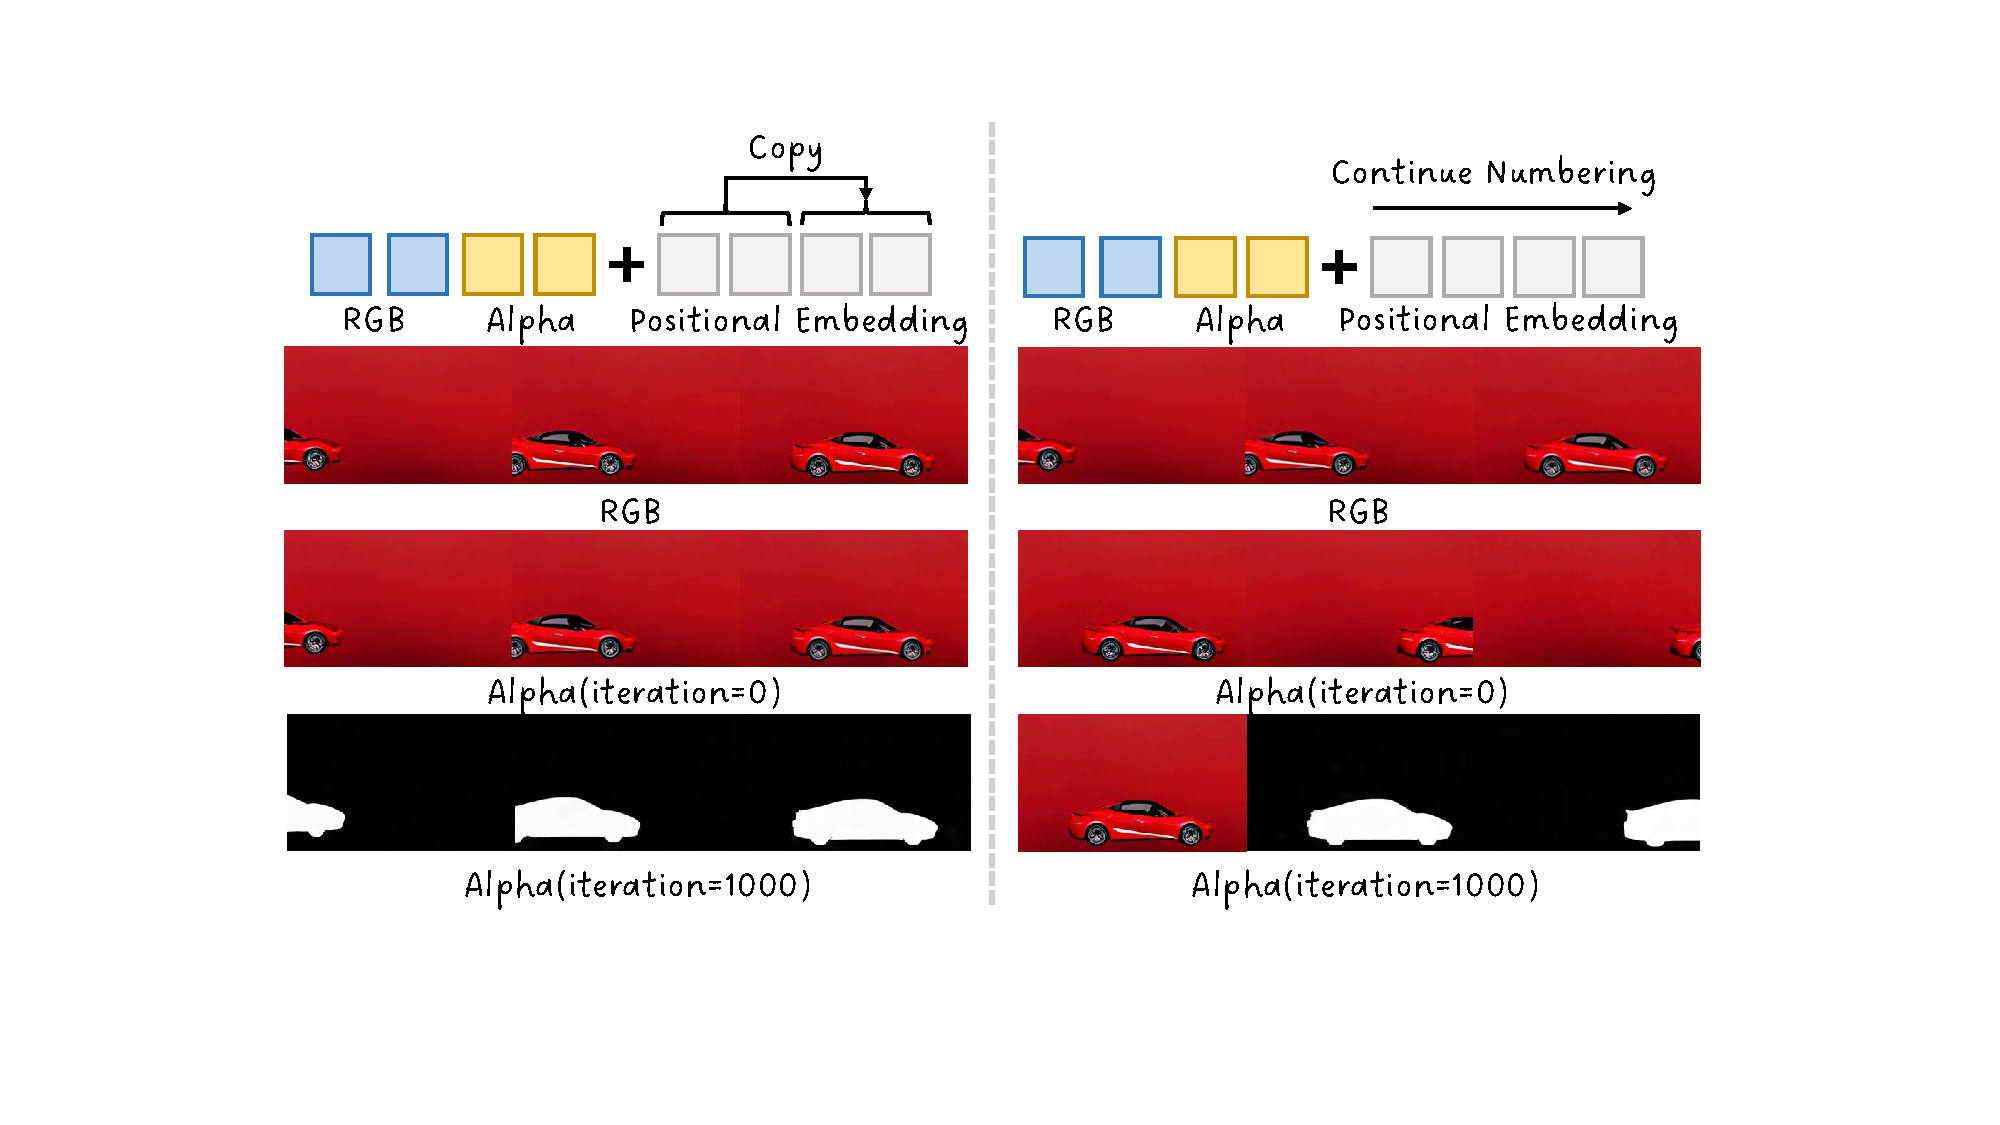
\includegraphics[width=1.0\linewidth]{figs/method-pe_init.pdf}
    \vspace{-0.2in}
    \caption{\textbf{Positional Encoding Design for RGBA Generation.} Assigning alpha tokens the same positional encoding as RGB yields similar results, resulting in faster convergence after 1000 iterations compared to standard encoding strategies.}
    \label{fig-pe}
    \vspace{-0.1in}
\end{figure}

% %-------------------------------------------------------------------------
\subsection{Analysis}
% % given our goal is 最大程度地继承 pretrain video model的能力,让它能生成的东西超越已有的RGBA训练集,
% 在目前我们使用的3d full attention DiT的video generation model的框架下,最重要的计算是attention mechanism,因此我们进一步对该过程进行分析:
% The attention matrix, \(\mathbf{Q}\mathbf{K}^T\), now has dimensions \((L_\text{text} + 2*L) \times (L_\text{text} + 2*L)\), which we simplify by organizing it into a 3x3 grouped attention matrix—\textbf{Text-attend-to-RGB}, \textbf{RGB-attend-to-Text}, and so forth, as illustrated in Fig.~\ref{fig-pipeline}. Then we procceed to analyze them:

% \noindent{\textbf{Text-Attend-to-RGB} and \textbf{RGB-Attend-to-Text}}.
% Given this matrix, we are supposed to preserve as much of the computation in the upper-left 2x2 section as possible so that we can preserve the RGB generation potential. 

% These represent the upper-left 2x2 section in \(\mathbf{Q}\mathbf{K}^T\) and 是RGB original generation model有且仅有的计算过程,如果我们能保证这部分计算不受影响,we can replicate the original RGB generation performance. 
% Therefore, we limited the scope of LoRA's influence, as defined in Equation~\eqref{eq:our_lora}, we retain the original QKV values for both text and RGB tokens, maintaining the pretrained model’s behavior in these domains.

% Besides the partial lora, the introduction of alpha tokens make the text and RGB tokens need to act as key and interact with alpha tokens as query, which will also 改变这个2x2 attention matrix的计算结果。
% Therefore, we proceed to analyze two additional attention computations that affect RGB generation shown in Fig.~\ref{fig-attn}:


% \noindent{\textbf{Text-Attend-to-Alpha}}: We find this attention is detrimental to the generation quality. 
% Since the model is originally trained with text and RGB data, introducing attention from text to alpha causes interference due to the domain gap between alpha and RGB. 
% Specifically, alpha modality provide only contour information and lack the rich texture, color, and semantic details associated with text prompt, thereby degrading generation quality. 
% To mitigate this, we design the attention mask (Equation~\eqref{eq:attn_mask}) that blocks this computation.

% \noindent{\textbf{RGB-Attend-to-Alpha}}: In contrast, we identify \textbf{RGB-to-Alpha} as essential for successful joint generation. 
% This attention allows the model to refine RGB tokens by considering alpha information, facilitating alignment between generated RGB and alpha channels. 
% This refinement process is a critical component missing in prior generation-then-prediction pipelines, which lack a feedback mechanism for RGB refinement based on alpha guidance.
Given our goal of maximizing the inherited capabilities of the pretrained video model, enabling it to generate beyond the existing RGBA training set, we analyze the most critical component within our current 3D full attention DiT video generation model: the attention mechanism.
%
The attention matrix, \(\mathbf{Q}\mathbf{K}^T\), has dimensions \((L_\text{text} + 2*L) \times (L_\text{text} + 2*L)\), which we simplify by organizing it into a 3x3 grouped attention matrix—including \textbf{Text-attend-to-RGB}, \textbf{RGB-attend-to-Text}, and so forth, as illustrated in Fig.~\ref{fig-pipeline}. %We then analyze these components:

\vspace{0.5em}
\noindent\textbf{Text-Attend-to-RGB and RGB-Attend-to-Text}. These represent the upper-left 2x2 section of  and are computations that exist solely in the original RGB generation model. If we ensure that this part of the computation remains unaffected, we can replicate the original RGB generation performance. Therefore, we limit the scope of LoRA's influence, as defined in Eq.~\eqref{eq:attn_mask}, by retaining the original QKV values for both text and RGB tokens, thus preserving the pretrained model’s behavior in these domains.

Besides the partial LoRA, the added alpha tokens requires the text and RGB tokens to also act as queries and interact with the alpha tokens as keys, which alters the computation in this 2x2 attention matrix. 
Therefore, we further analyze two additional attention computations that impact RGB generation, as shown in Fig.~\ref{fig-attn}.

\vspace{0.5em}
\noindent\textbf{Text-Attend-to-Alpha.} We find that this attention is detrimental to the generation quality. Since the model was originally trained with text and RGB data, introducing attention from text to alpha causes interference due to the domain gap between alpha and RGB. Specifically, the alpha modality provides only contour information and lacks the rich texture, color, and semantic details associated with the text prompt, thereby degrading generation quality. To mitigate this, we design the attention mask (Eq.~\eqref{eq:attn_mask}) that blocks this computation.

\vspace{0.5em}
\noindent\textbf{RGB-Attend-to-Alpha.} In contrast, we identify \textbf{RGB-to-Alpha} as essential for successful joint generation. This attention allows the model to refine RGB tokens by considering alpha information, facilitating alignment between generated RGB and alpha channels. This refinement process is a critical component missing in previous generation-then-prediction pipelines, which lacked a feedback mechanism for RGB refinement based on alpha guidance.


\begin{figure}[t]
    \centering
    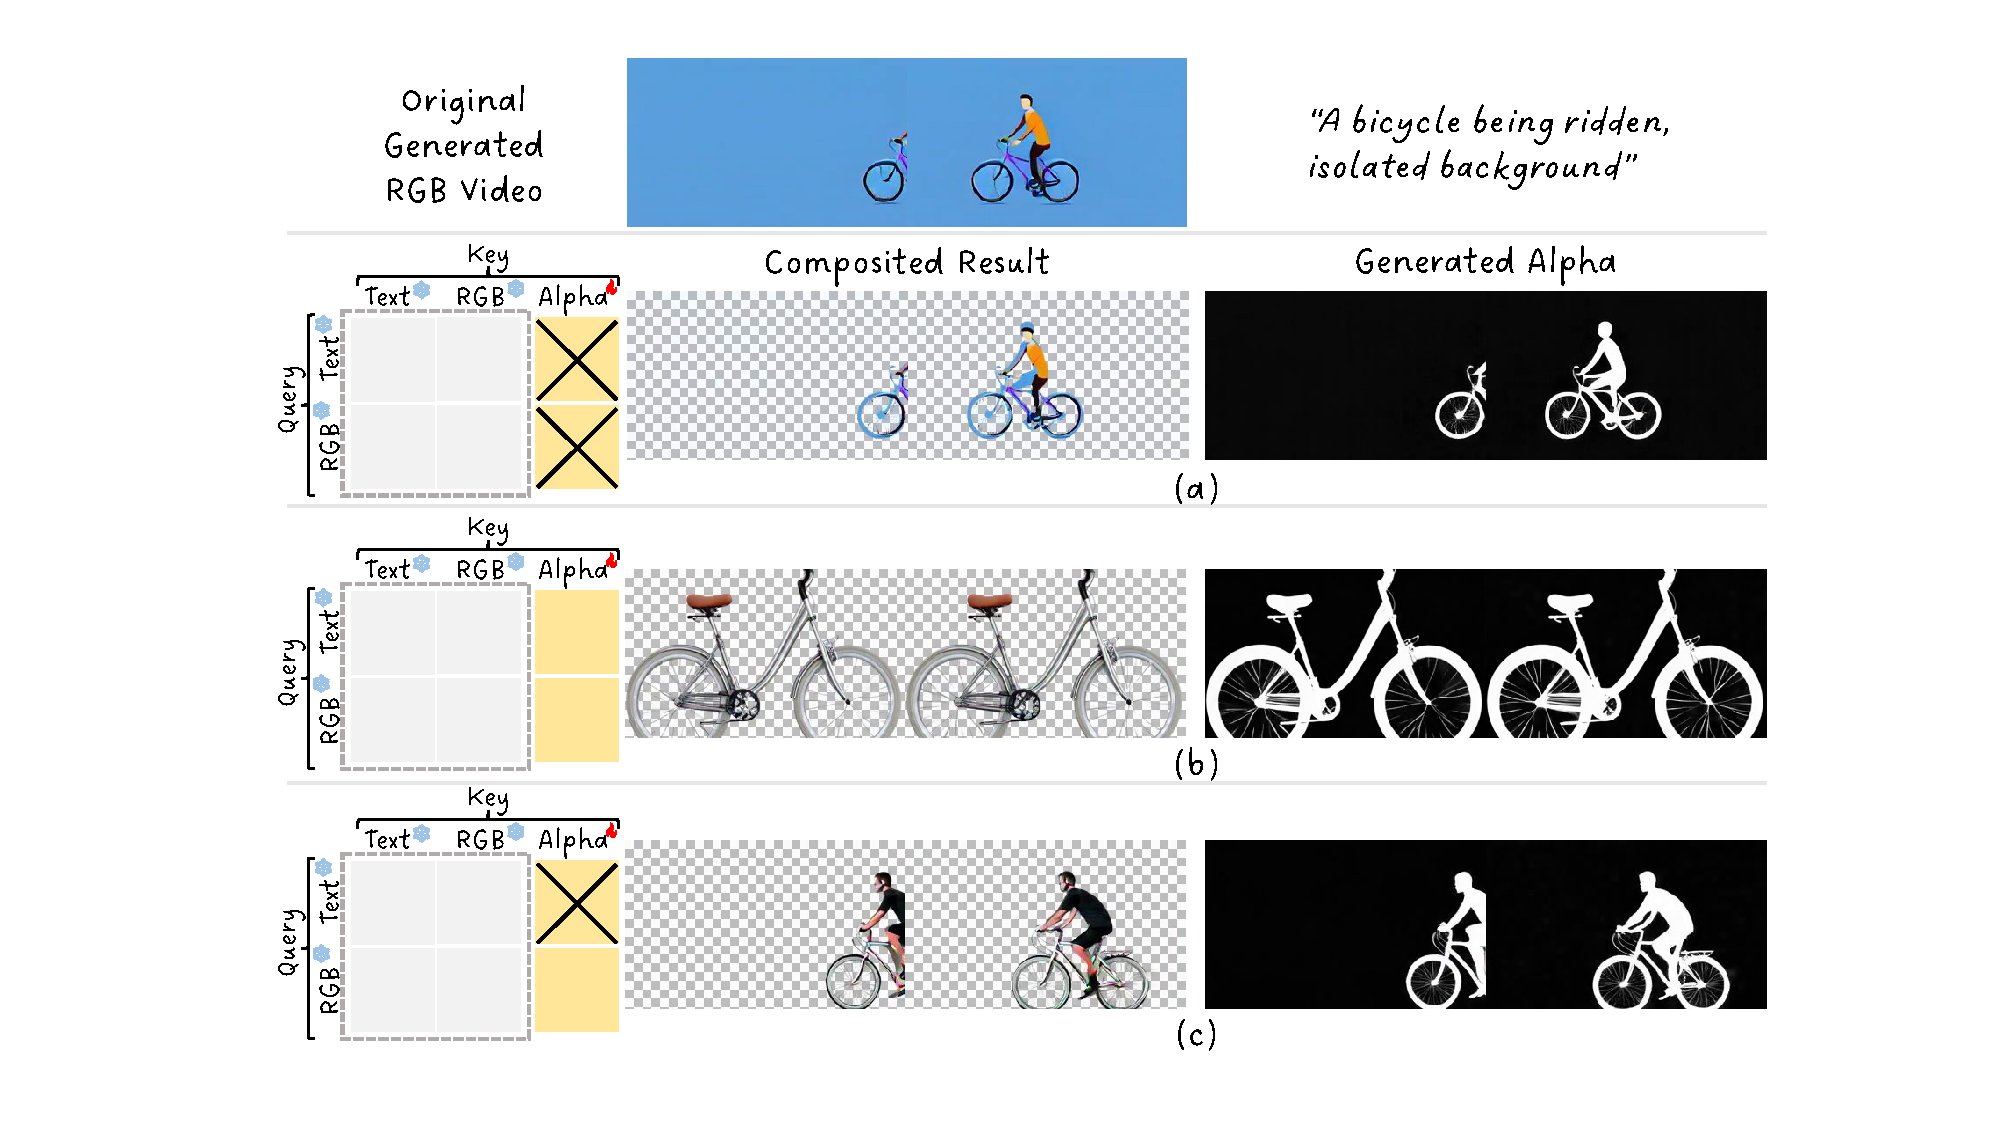
\includegraphics[width=1.0\linewidth]{figs/method-attn.pdf}
    \vspace{-0.2in}
    \caption{\textbf{Attention Rectification.} (a) Eliminating all attention from alpha as a key preserves 100\% RGB generation but leads to poor alignment. (b) Retaining all attention significantly degrades quality, causing a lack of motion in bicycles. (c) Our method achieves an effective balance.
    }
    \label{fig-attn}
    \vspace{-0.1in}
\end{figure}




%
% --- inline annotations
%
\newcommand{\red}[1]{{\color{red}#1}}
\newcommand{\todo}[1]{{\color{red}#1}}
\newcommand{\TODO}[1]{\textbf{\color{red}[TODO: #1]}}
% --- disable by uncommenting  
% \renewcommand{\TODO}[1]{}
% \renewcommand{\todo}[1]{#1}

\usepackage{xcolor}
\usepackage{graphicx}
\usepackage{booktabs}
\usepackage{amsmath} 
\usepackage{amsfonts}
\usepackage{amssymb}
\usepackage{multirow} 
\usepackage{makecell}
\newcommand{\shline}{\Xhline{1.1pt}} % Adjust thickness as desired

\section{Experiments}
\label{sec:experiments}

We present results for supervised video classification and self-supervised masked auto-encoding with frozen representations evaluated on two downstream tasks: video classification and point tracking. To analyse the memory capabilities of our model, we also include a reconstruction task of frames seen in the distant past. Using the same task, we study the generalisation capabilities to longer sequences than seen during training. We follow the ViT scaling configurations and, unless otherwise stated, we use the \textbf{B}ase version for our model for all our experiments. We specify the number of parameters for all models considered in our experiments, and we include in the supplementary material all the training hyperparameters and data augmentations used in all experiments.

\subsection{Supervised video classification}

\par \noindent \textbf{Datasets:}
We use large-scale real-world datasets for the supervised video classification task. Kinetics400~\citep{Carreira_2017_CVPR} contains 241,512 videos\footnote{Kinetics is a dynamic dataset (videos may be removed from
YouTube). Our current version has 241,512 videos, compared to 267,000 videos reported in~\cite{vivit}, so a decrease of almost 10\%, noticeable in the final performance.} across train, validation, and test splits, 10s-long (25fps), spanning 400 classes. This dataset is known to require modelling appearance for successful action recognition. To challenge our model's capability of understanding motion, we also use SSv2 dataset~\citep{goyal2017something}, which contains 220,847 shorter videos (2-6s long), sampled at 12fps, representing 174 classes. This dataset includes actions that differ in finer motion-related details, requiring a deeper temporal understanding, e.g. \textit{pouring something into something} vs \textit{pretending to pour something into something}. 

\par \noindent \textbf{Baselines:}
We use ViViT~\citep{vivit} as our main baseline. We consider the full self-attention version, which patchifies and flattens the entire video, prepends a video class token, then runs self-attention blocks. We also consider the factorised encoder version (ViViT FE), which runs a ViT image model over all the frames, and uses temporal self-attention blocks to integrate the information over time. Finally, we also consider a baseline that uses only LRU recurrent and MLP blocks, configured similar to VideoMamba~\cite{li2024videomambastatespacemodel}, i.e. it does not use self-attention blocks, denoted \textit{PureLRU}. Similar to ViViT, this model first patchifies and flattens the video, prepends a class token, then applies a sequence of recurrent blocks. All baselines use learnt spatio-temporal positional encoding, whereas the proposed \ssm\ uses only spatial positional encoding as the temporal dimension is implicitly modelled through its recurrence.


\par \noindent \textbf{Results:} We include results for training from scratch or using Imagenet pre-trained weights to initialise the weights of the ViT blocks. Figure~\ref{fig:baselines} shows a first comparison between \ssm\ and the above baselines, with all models being trained from scratch on supervised classification on SSv2. We consider the \textbf{S}mall version for all models as the larger \textbf{B}ase version shows stability issues when trained from scratch, as reported in other works as well~\cite{li2024videomambastatespacemodel,vivit}. As expected, the performance on this challenging dataset when training from scratch is far from SOTA, but it clearly shows that the proposed factorisation has superior video modelling capabilities compared to baselines, ViViT-S with full self-attention being the closest competitor. PureLRU's performance is very poor, which is in line with the findings of other works (\eg VideoMamba) who report that bidirectional (non-causal) processing of the input is needed for good performance. 

We report further results comparing against ViViT-B and ViViT-L with full self-attention when using Imagenet pre-trained weights; see Table~\ref{tab:ssv2} for SSv2 results and Table~\ref{tab:kinetics} for Kinetics400 results.
We can observe that our model achieves better performance compared to ViViT baselines on SSv2, but it is slightly below ViViT-L on Kinetics400. This result could reflect the difference between the two datasets mentioned above: outperforming ViViT-L on SSv2 suggests that \ssm\ is superior at modelling motion compared to ViViT, but on Kinetics where the appearance is enough for successful classification, both models are on par. We consider this to be a strong positive result for our model given that it has about 3x less parameters compared to ViViT-L and significantly lower FLOPs count and memory footprint as shown in Figure~\ref{fig:memory}.

\begin{figure}[t]
  \centering
  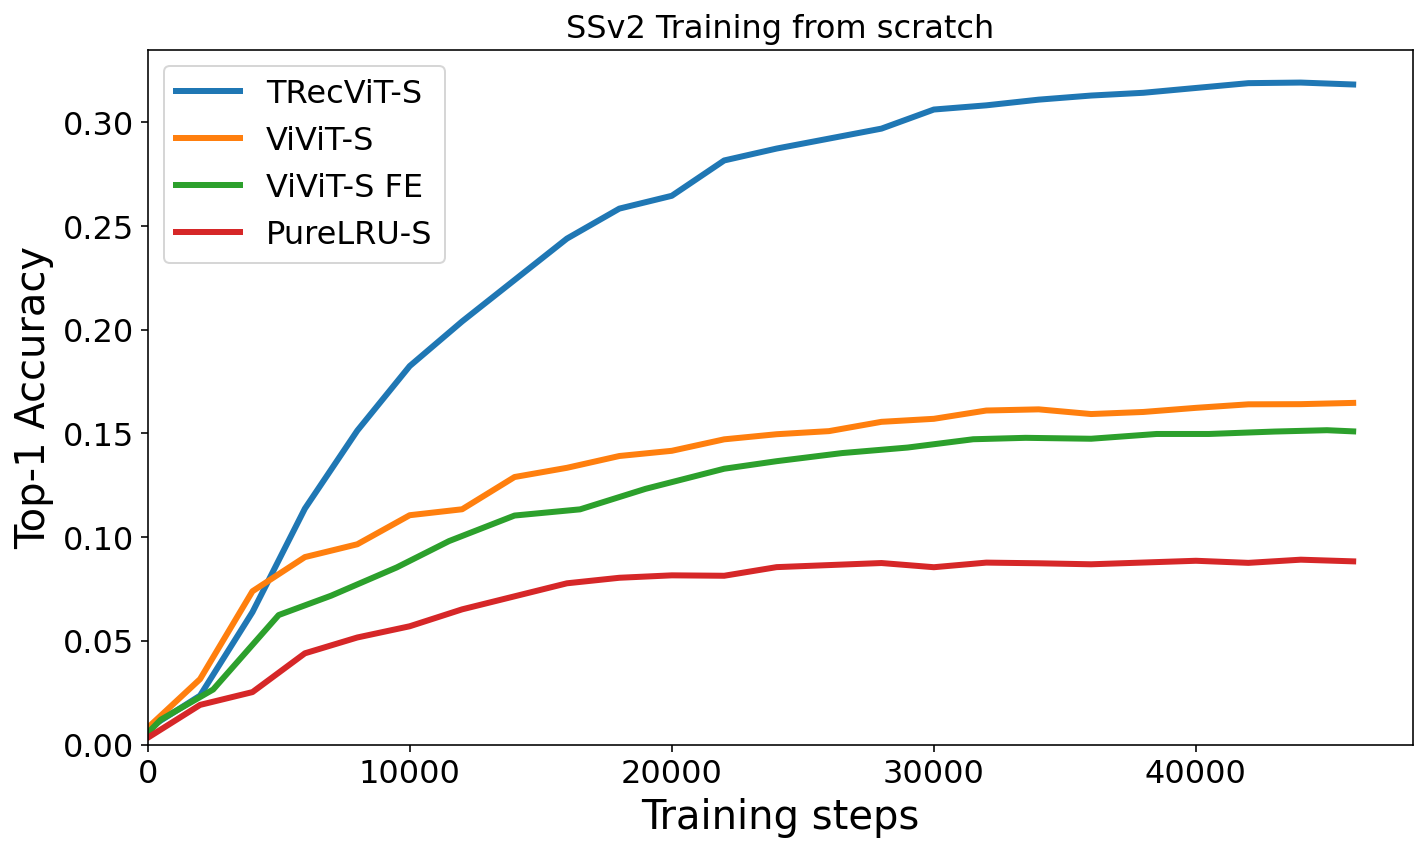
\includegraphics[width=.9\linewidth]{img/scratch.png}
  \caption{\ssm\ compared to baselines on supervised video classification on SSv2 dataset, trained from scratch. The plot shows the evolution of the evaluation accuracy as training progresses.
  }

  \label{fig:baselines}
\end{figure}
 

 \begin{figure*}[h]
  \centering
  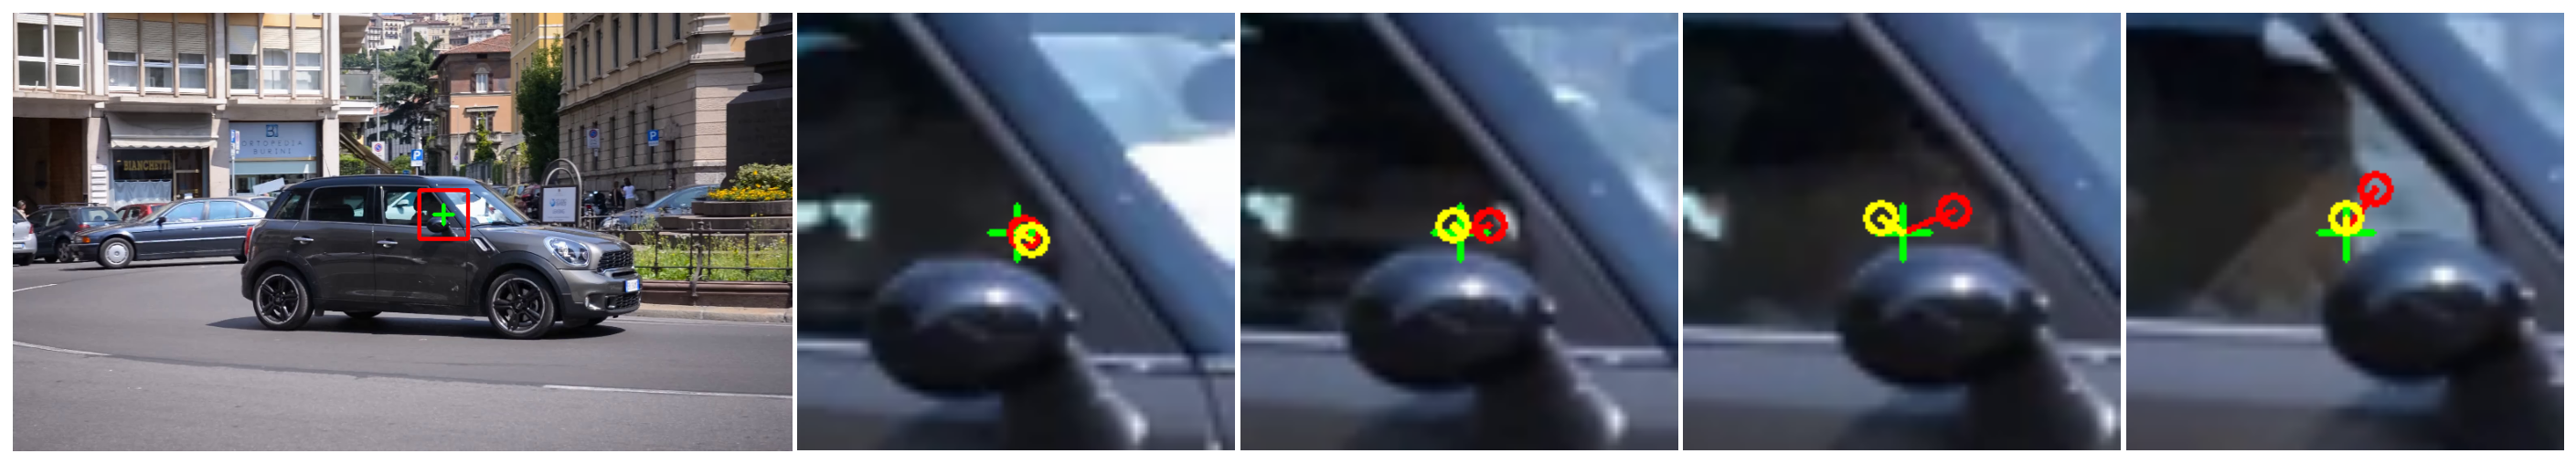
\includegraphics[width=\linewidth]{img/davis.png}
  \caption{Qualitative results obtained by \ssm\ for point tracking on DAVIS dataset compared to VideoMAE. The leftmost image indicates the point to track in the original frame, and the images towards the right show zoom-ins on subsequent frames. Green plus (+) marker indicates the ground truth, yellow circle indicates \ssm's predictions and red circles indicate VideoMAE's predictions.}
  \label{fig:tracking}
\end{figure*}


\begin{table}
    \centering
    \small{
    \begin{tabular}{l|c|c|r}
    \hline
    \textbf{Model} & \textbf{Patch size} & \textbf{Top-1 acc (\%)} & \textbf{\# params} \\
    \hline
    ViViT-B & (2, 16, 16) & 59.1 & 90M \\
    ViViT-L & (2, 16, 16) & 65.9 & 320M \\
    \ssm\ & (1, 16, 16) & \textbf{66.8} & 109M\\
    \hline
    \end{tabular}}
    \caption{Performance of \ssm\ compared to ViViT-B and ViViT-L baselines on SSv2 dataset with all models initialised from Imagenet pre-training. For ViViT-L, we use the result reported by its authors, for ViViT-B we obtained the results internally as they were not reported in the original paper for this dataset.}
    \label{tab:ssv2}
    \end{table}
    
\begin{table}
    \centering
    \small{
    \begin{tabular}{l|c|c|r}
    \hline
    \textbf{Model} & \textbf{Patch size} & \textbf{Top-1 acc (\%)} & \textbf{\# params} \\
    \hline
    ViViT-B & (2, 16, 16) & 78.1 & 90M \\
    ViViT-L & (2, 16, 16) & \textbf{78.7} & 320M \\
    \ssm\ & (1, 16, 16) & 78.4 & 109M\\
    \hline
    \end{tabular}}
    \caption{Performance of \ssm\ compared to ViViT-B and ViViT-L baselines on Kinetics400 dataset, with all models initialised from Imagenet pre-training. For ViViT-B and ViViT-L, we include the result we obtained internally by re-training the model on the current Kinetics400 dataset version; see footnote. In the original paper, the authors reported 80.3\% on Kinetics400 for ViViT-L.}
    \label{tab:kinetics}
    \end{table}

\subsection{Self-supervised masked autoencoding}
\label{sec:mae}
We use Kinetics400 for self-supervised pre-training from scratch and we report results on multiple downstream datasets and tasks by fine-tuning attention readout heads on top of frozen representations. We choose this setup, as opposed to fine-tuning end-to-end, as the  performance in this case more clearly reflects the quality of the pre-trained representations. As mentioned in the previous section, we use a large masking ratio (0.90), which makes pre-training very efficient. We report the number of parameters for every model considered. Note that the number of parameters for \ssm\ is different from the one reported in the previous section due to the addition of the readout heads.

\par \noindent \textbf{Video classification:}  We report video classification accuracy as downstream task using attention readout heads on SSv2 and Kinetics400. We compare the performance against VideoMAE-L~\cite{tong2022videomae} in Table~\ref{tab:selfsup}. Our model obtains slightly better performance on both datasets compared to this strong baseline, despite having almost 3$\times$ less parameters. 

\par \noindent \textbf{Point tracking:} To demonstrate that our model can handle dense(r) tasks as well, we evaluate the same frozen MAE representations for the point tracking task. We use the recurrent architecture in MooG~\cite{steenkiste2024moving} as a readout due to its simplicity. MooG uses light cross-attention layers to process the embeddings of each frame in order, and the readout state is carried over through time. We finetune the MooG readout head using MOVi-E dataset~\cite{movie} as done in popular point tracking works~\cite{DoerschYVG0ACZ23}. We evaluate these fine-tuned representations on two datasets: Perception Test~\citep{patraucean2023perception} and DAVIS dataset~\cite{davis2017} with point tracks extracted in~\cite{doersch2022tapvid}. We report average Jaccard metric~\cite{doersch2022tapvid} for \ssm\ compared with MooG and VideoMAE; see Table~\ref{tab:pt}. \ssm\ obtains better performance on both datasets compared to baselines, which reinforces the observation that our proposed model has strong motion modelling capabilities. We include qualitative results for this task in Figure~\ref{fig:tracking}. We can observe that the results are visibly better compared to VideoMAE. More visualisations are included in the supplementary material.

\begin{table}
    \centering
    \small{
    \begin{tabular}{l|c|c|r}
    \hline
    \textbf{Model} & \textbf{Dataset} & \textbf{Top-1 acc (\%)} & \textbf{\# params} \\
    \hline
    VideoMAE & Kinetics400 & 45.8 & 330M \\
    \ssm\ & Kinetics400 & \textbf{46.0} & 128M\\
    \hline
    \hline
    VideoMAE & SSv2 &  53.7 & 330M \\
    \ssm\ & SSv2 &  \textbf{53.9} & 128M\\
    \hline
    \end{tabular}}
    \caption{Performance of \ssm\ compared to VideoMAE on video classification using frozen MAE representations, pre-trained on Kinetics400.}
    \label{tab:selfsup}
    \end{table}

\begin{table}
    \centering
    \small{
    \begin{tabular}{l|c|c|c|r}
    \hline
    \textbf{Model} & \textbf{Dataset} & \textbf{\# frames} & \textbf{AJ} & \textbf{\# params} \\
    \hline
    MooG & DAVIS & 8 & 0.687 & 35M \\
    VideoMAE & DAVIS & 8 & 0.703 & 330M \\
    \ssm\ & DAVIS & 8 & \textbf{0.706} & 128M\\
    
    \hline
    \hline
    MooG & Perception Test & 16 & 0.760 & 46.5M \\
    VideoMAE & Perception Test & 16 & 0.761 & 330M \\
    \ssm\ & Perception Test & 16 & \textbf{0.783} & 128M\\
    \hline
    \end{tabular}}
    \caption{Performance of \ssm\ compared to baselines on point tracking task on DAVIS and Perception Test datasets. All models use frozen representations evaluated using the readout head from MooG.}
    \label{tab:pt}
    \end{table}

\begin{figure*}[h]
  \centering
  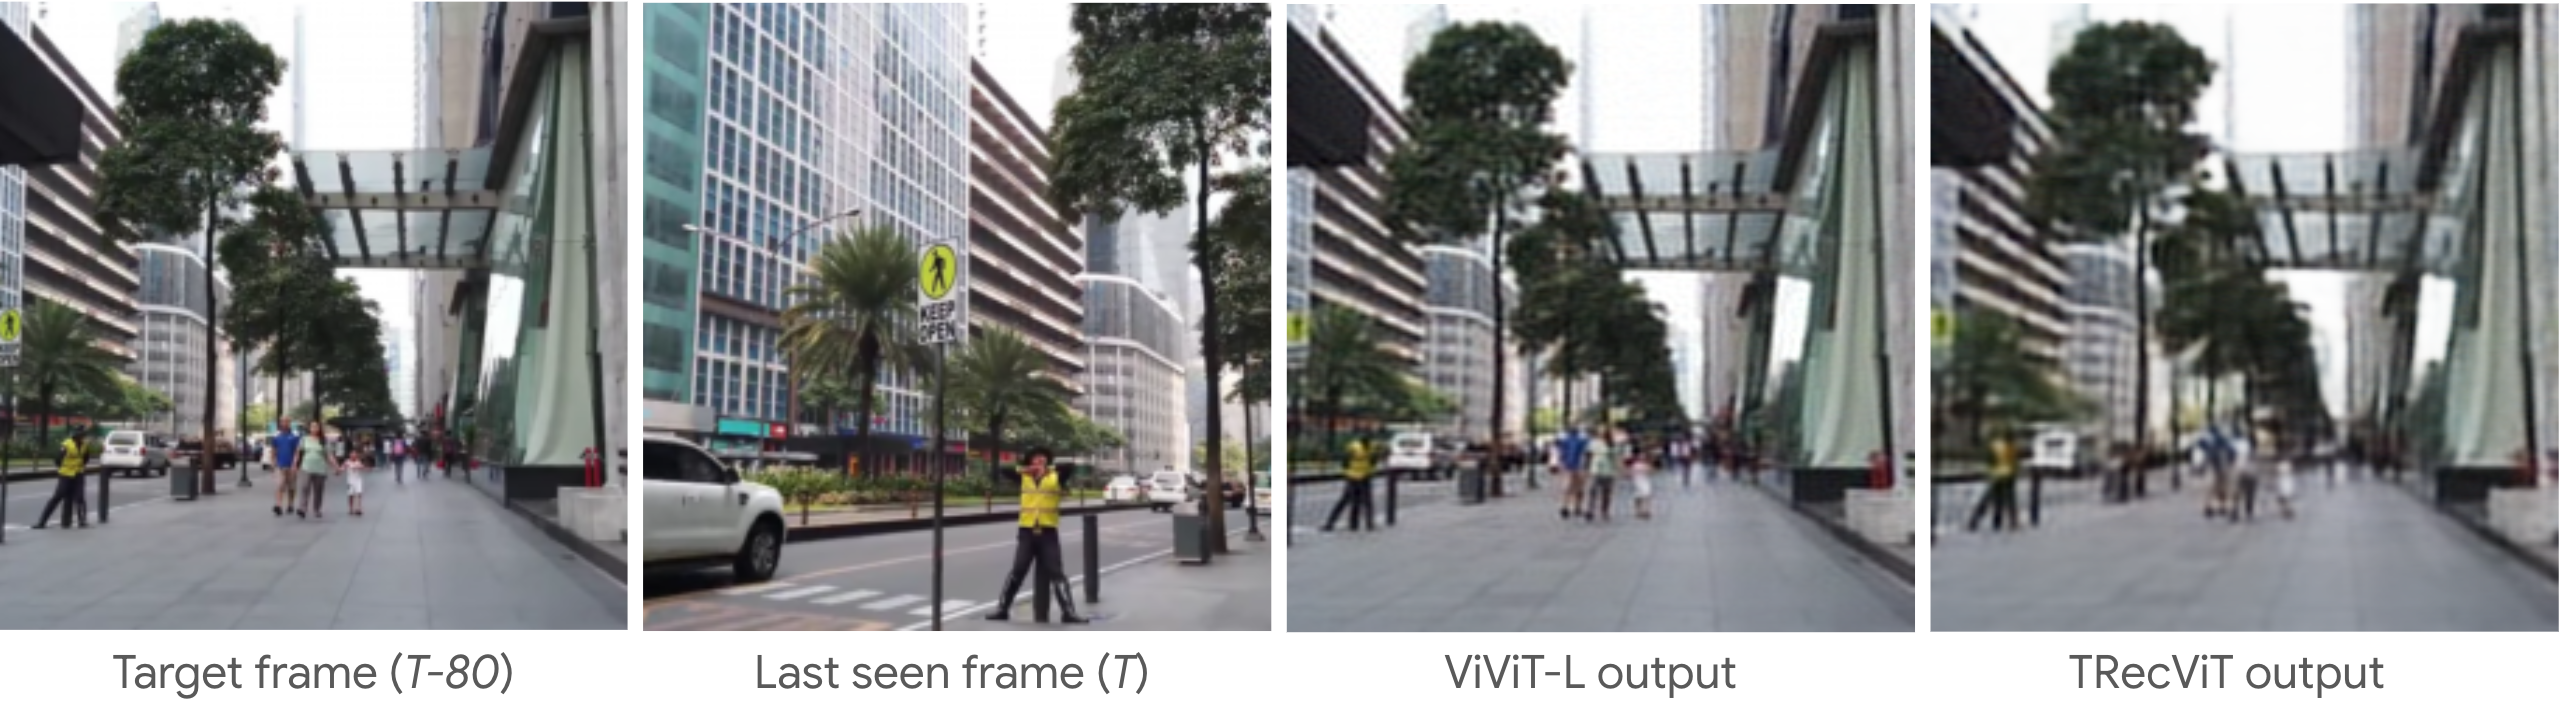
\includegraphics[width=\linewidth]{img/wtlong.png}
  \caption{Qualitative results obtained by \ssm\ on the dense memorisation task compared to ViViT-L. Both models are trained using Imagenet pre-trained weights, on video sequences of $T=64$ frames and they reconstruct the $(T-48)^\text{th}$ frame.}
  \label{fig:wt}
\end{figure*}

\begin{figure}[t]
\centering
\begin{subfigure}{0.48\linewidth}
    \centering
    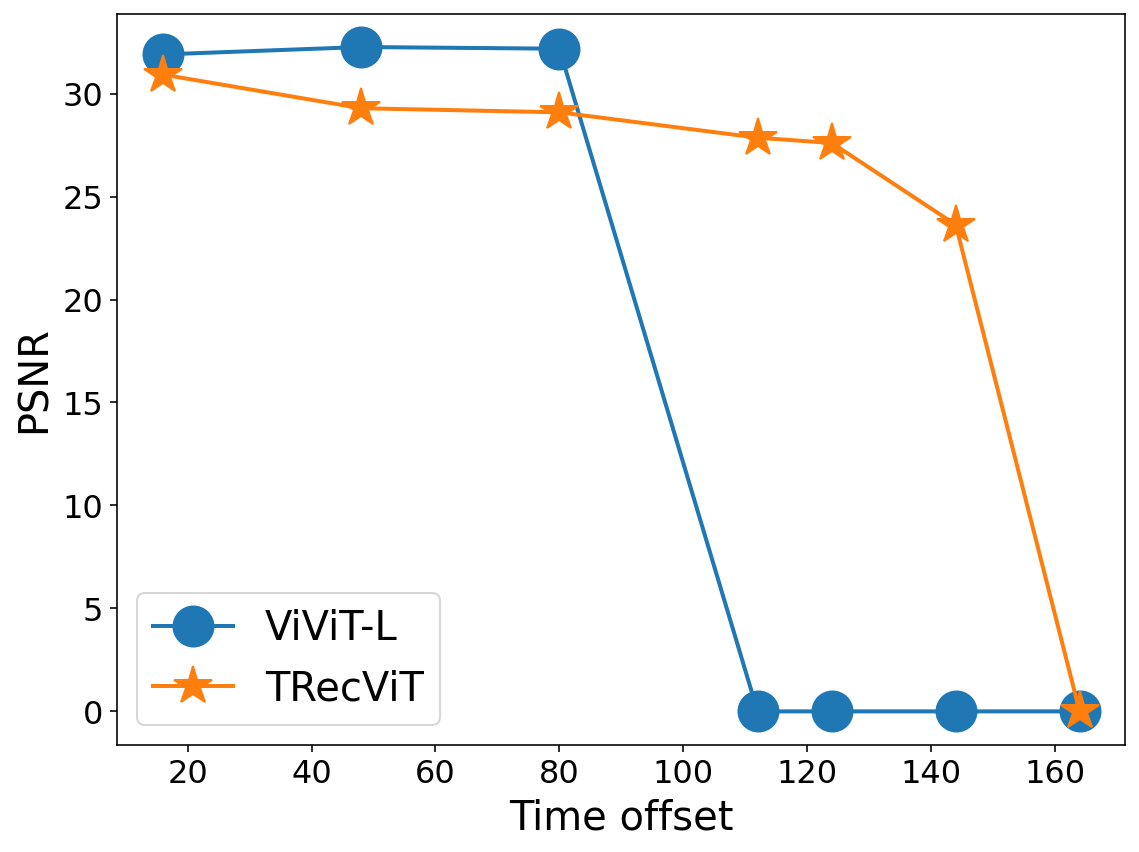
\includegraphics[width=\textwidth]{img/psnr.png}
    \caption{PSNR comparison}
\end{subfigure}%
\hfill
\begin{subfigure}{0.48\linewidth}
    \centering
    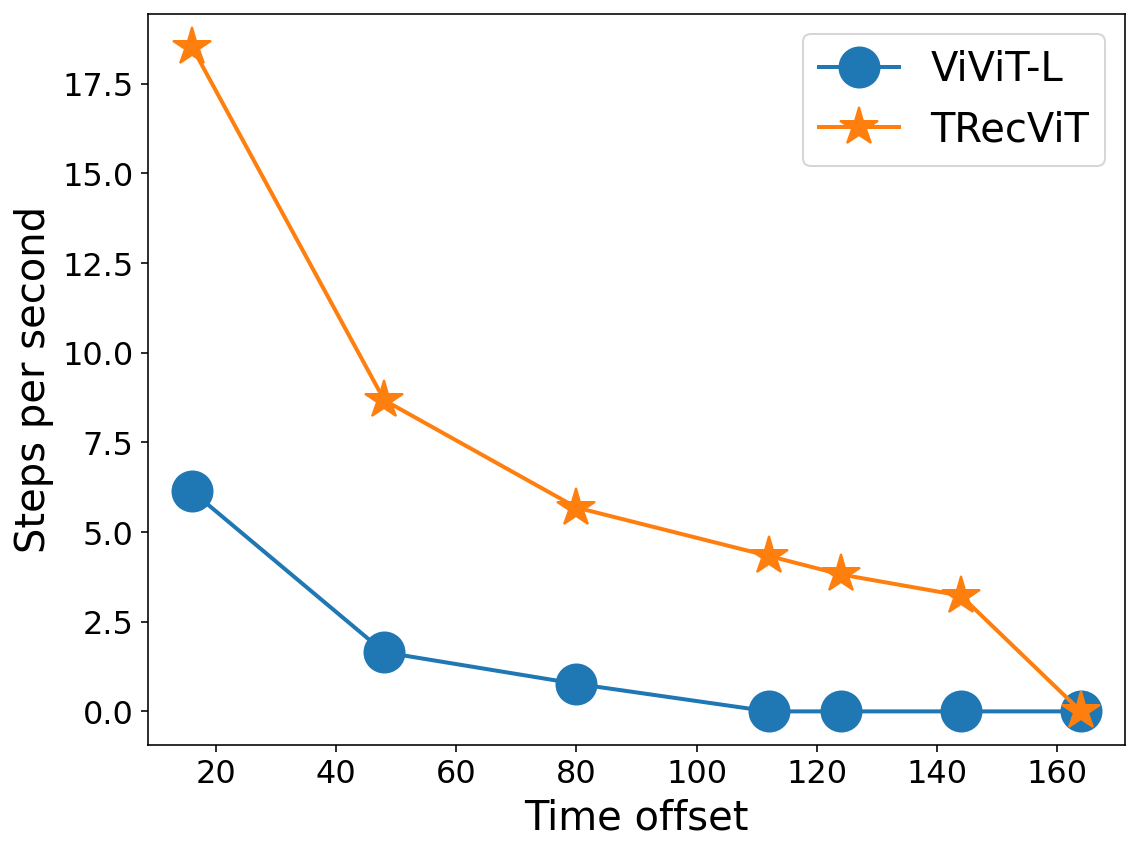
\includegraphics[width=\textwidth]{img/sps.png} 
    \caption{Steps-per-second comparison}
\end{subfigure}
\caption{Long video memorisation task. At time $T$, the model has to reconstruct the $(T-k)^\text{th}$ frame seen in the past. The plots show PSNR and throughput (steps-per-second) for increasing time offset $k$. For both models, the data points with $0$ value on the $y$-axis correspond to OOM.
}
\label{fig:psnr}
\end{figure}

\subsection{Long video memorisation task}
\label{sec:longtask}

Transformer models for language are known to be excellent at retrieving information from context, as they cache the keys and values for the entire history. On the other hand, LRUs / SSMs and RNNs in general struggle with such \emph{needle-in-the-haystack} style tasks as they need to perform the retrieval based on the compressed history kept in their recurrent state~\cite{jelassi2024repeat, de2024griffinmixinggatedlinear}. 
We are interested in studying this aspect in the video domain as well. We set up a simple reconstruction task where the model has to remember the frame seen at a given time-step in the past. For our analysis, we run multiple experiments where the model is tasked to reconstruct the $(T-k)^{\text{th}}$ frame from the past, with increasing value for $k\in\{16, 48, 80, 112, 144, 164\}$ frames. We employ Walking Tours dataset~\cite{venkataramanan2023imagenet}, which contains hour-long videos, and the scenery changes constantly, hence we are guaranteed that the video frames seen most recently will be very different compared to the frames seen earlier on. We scale the videos to $224\times224$ pixels. Again, we adopt ViViT-L as baseline, and we train both models using Imagenet pretrained weights. For ViViT-L, we keep all the outputs from all $T$ time steps and apply temporal pooling and a $1\times1$ convolution to get the expected shape for the reconstructed frame. For \ssm, we simply keep the output of the last layer at time step $T$ and reshape it to the expected shape. We show quantitative and qualitative results respectively in Figures~\ref{fig:psnr} and~\ref{fig:wt}. We can observe that there is a performance--efficiency trade-off at play for \ssm: its performance is slightly below ViViT's for shorter memory spans (16, 48, 80), but its efficiency (steps-per-second) is significantly higher. However, beyond 80 frames, ViViT-L goes out of memory, whilst \ssm\ continues to give decent results up to 144 frames, going out of memory towards 164 frames. Figure~\ref{fig:wt} shows qualitative results compared to the baseline for the case where the models have to remember the frame seen at $T-48$ in the past. We can observe that the quality of ViViT-L's reconstruction is good. For \ssm, whilst the overall structure (encoded in lower frequencies) is correct, it struggles to remember the high-frequency content of the image. This is to be expected due to the compression happening in the recurrent state of the model. However, given how different the last seen frame is from the target frame, we consider this to be a very promising result that warrants further investigation into the memorisation capabilities of our model, which we leave as future work.

\subsection{Generalisation to longer sequences}
\label{sec:gentask}

Using the same task as above, we analyse the generalisation capabilities to sequences longer than those used during training. Specifically, we train the models with sequences of length $T=64$ frames to reconstruct the $T-48$ frame, and evaluate them on longer sequences $T=96$ to reconstruct the same frame. The \ssm\ model can run on longer sequences without any modification. For the ViViT model, we need to adapt the positional encoding to accommodate longer sequences. We use interpolation to nearest neighbour to obtain the desired length; cubic interpolation led to worse results. The performance of \ssm\ degrades slightly, with PSNR going down from 29.3 (when evaluated on the same sequence length as in training $T=64$) to 26.4 when evaluated with $T=96$ frame sequences. ViViT's PSNR, however, drops significantly, from 32.3 when evaluated on the same sequence length, to 15.1 when evaluated on longer sequences. We include qualitative examples in Figure~\ref{fig:gentask} where we can observe that ViViT's output contains stronger artefacts compared to \ssm. 

\begin{figure}[h]
  \centering
  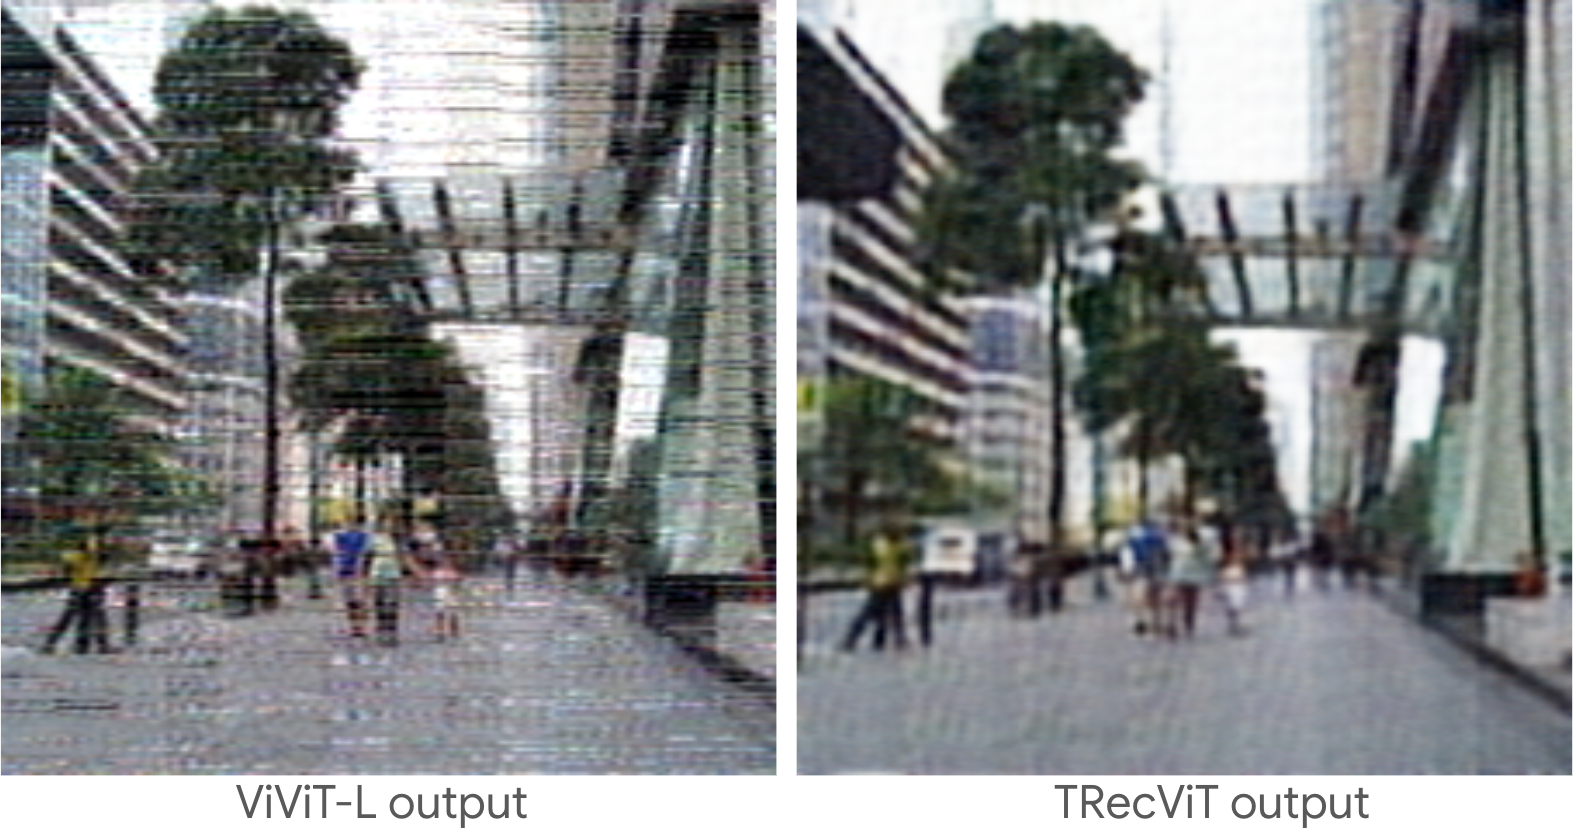
\includegraphics[width=\linewidth]{img/genlong.png}
  \caption{Generalisation to longer sequences. Both models are trained using Imagenet pre-trained weights, on video sequences of $T=64$ frames to reconstruct the $(T-48)^\text{th}$ frame; during evaluation, the models receive sequences of $T=96$ frames.}
  \label{fig:gentask}
\end{figure}

\vspace{-2mm}
\section{Analysis}
\label{sec:analysis}
\vspace{-1mm}

\subsection{Choice of diffusion framework}
\label{subsec:diffusion_choice}
\vspace{-1mm}

As explained in Section \ref{sec:framework}, we could in principle use any diffusion model variant in our world model. While \textsc{diamond} utilizes \textsc{edm} \citep{karras2022elucidating} as described in Section \ref{sec:method}, \textsc{ddpm} \citep{ho2020DDPM} would also be a natural candidate, having been used in many image generation applications \citep{ldm_stable_diffusion, ddpm++}. We justify this design decision in this section.

To provide a fair comparison of \textsc{ddpm} with our \textsc{edm} implementation, we train both variants with the same network architecture, on a shared static dataset of 100k frames collected with an expert policy on the game \textit{Breakout}. As discussed in Section \ref{subsec:dwm_training}, the number of denoising steps is directly related to the inference cost of the world model, and so fewer steps will reduce the cost of training an agent on imagined trajectories. \citet{ho2020DDPM} use a thousand denoising steps, and \citet{ldm_stable_diffusion} employ hundreds steps for Stable Diffusion. However, for our world model to be computationally comparable with other world model baselines (such as \textsc{iris} which requires 16 NFE for each timestep), we need at most tens of denoising steps, and preferably fewer. Unfortunately, if the number of denoising steps is set too low, the visual quality will degrade, leading to compounding error. 

To investigate the stability of the diffusion variants, we display imagined trajectories generated autoregressively up to $t=1000$ timesteps in Figure \ref{fig:denoising_trajectories}, for different numbers of denoising steps $n \le 10$. We see that using \textsc{ddpm} (Figure \ref{fig:denoising_with_ddpm}) in this regime leads to severe compounding error, causing the world model to quickly drift out of distribution. In contrast, the \textsc{edm}-based diffusion world model (Figure \ref{fig:denoising_with_karras}) appears much more stable over long time horizons, even for a single denoising step. A quantitative analysis of this compounding error is provided in Appendix~\ref{app:ddpm_drift}.

% %%%%%%%%%%%%%%%%%%%%%%%
\begin{figure}[h]
  \begin{subfigure}{0.49\linewidth}
    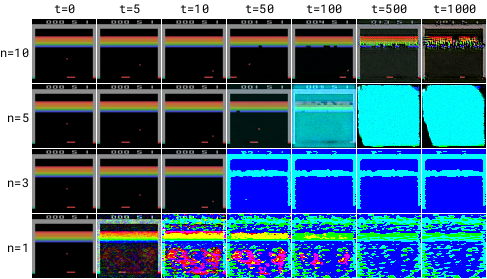
\includegraphics[width=\linewidth]{images/figure__karras_vs_ddpm__ddpm.png}
    \caption{\textsc{ddpm}-based world model trajectories.} \label{fig:denoising_with_ddpm}
  \end{subfigure}%
  \hspace*{\fill}   % maximize separation between the subfigures
  \begin{subfigure}{0.49\textwidth}
    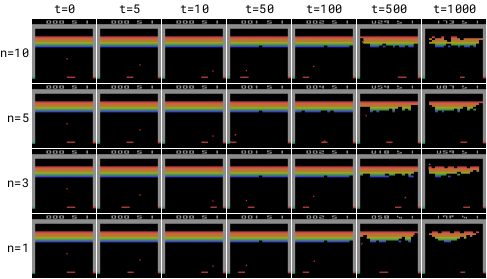
\includegraphics[width=\linewidth]{images/figure__karras_vs_ddpm__karras.png}
    \caption{\textsc{edm}-based world model trajectories.} \label{fig:denoising_with_karras}
  \end{subfigure}%

\caption{Imagined trajectories with diffusion world models based on \textsc{ddpm} (left) and \textsc{edm} (right). The initial observation at $t=0$ is common, and each row corresponds to a decreasing number of denoising steps $n$. We observe that \textsc{ddpm}-based generation suffers from compounding error, and that the smaller the number of denoising steps, the faster the error accumulates. In contrast, our \textsc{edm}-based world model appears much more stable, even for $n=1$.\vspace{-5mm}}
\label{fig:denoising_trajectories} 
\end{figure}
% %%%%%%%%%%%%%%%%%%%%%%%

This surprising result is a consequence of the improved training objective described in Equation~\ref{eq:effective_obj}, compared to the simpler noise prediction objective employed by \textsc{ddpm}. While predicting the noise works well for intermediate noise levels, this objective causes the model to learn the identity function when the noise is dominant ($\sigma_{noise}\gg\sigma_{data} \implies \xi_\theta(\x^\tau_{t+1}, y_t^\tau)\to\mathbf{x}^\tau_{t+1}$), where $\xi_\theta$ is the noise prediction network of \textsc{ddpm}. This gives a poor estimate of the score function at the beginning of the sampling procedure, which degrades the generation quality and leads to compounding error.

In contrast, the adaptive mixing of signal and noise employed by \textsc{edm}, described in Section \ref{subsec:practical_dwm}, means that the model is trained to predict the clean image when the noise is dominant ($\sigma_{noise}\gg\sigma_{data} \implies \mathbf{F_\theta}(\mathbf{x}^\tau_{t+1},y_t^\tau)\to\mathbf{x}^0_{t+1}$). This gives a better estimate of the score function in the absence of signal, so the model is able to produce higher quality generations with fewer denoising steps, as illustrated in Figure \ref{fig:denoising_with_karras}.


\subsection{Choice of the number of denoising steps}\label{subsec:denoising_steps}

 While we found that our \textsc{edm}-based world model was very stable with just a single denoising step, as shown for \textit{Breakout} in the last row of Figure \ref{fig:denoising_with_karras}, we discuss here how this choice would limit the visual quality of the model in some cases. We provide more a quantitative analysis in Appendix~\ref{app:denoising_ablation}.

As discussed in Section \ref{subsec:diffusion}, our score model is equivalent to a denoising autoencoder \citep{vincent2008extracting} trained with an $L_2$ reconstruction loss. The optimal single-step prediction is thus the expectation over possible reconstructions for a given noisy input, which can be out of distribution if this posterior distribution is multimodal. While some games like \textit{Breakout} have deterministic transitions that can be accurately modeled with a single denoising step (see Figure \ref{fig:denoising_with_karras}), in some other games partial observability gives rise to multimodal observation distributions. In this case, an iterative solver is necessary to drive the sampling procedure towards a particular mode, as illustrated in the game \textit{Boxing} in Figure \ref{fig:too_optimisitic_4_sure}. As a result, we therefore set $n=3$ in all of our experiments.
\vspace{-2mm}
%%%%%%%%%%%%%%%%%%%%%%%
\begin{figure}[h!]
%\vspace{-6mm}
\begin{center}
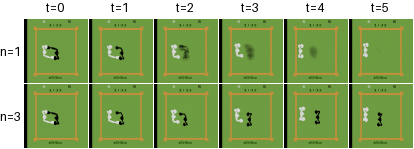
\includegraphics[width=.64\linewidth]{images/figure__blurry_boxing.png}
\caption{Single-step (top row) versus multi-step (bottom row) sampling in \textit{Boxing}. Movements of the black player are unpredictable, so that single-step denoising interpolates between possible outcomes and results in blurry predictions. In contrast, multi-step sampling produces a crisp image by driving the generation towards a particular mode. Interestingly, the policy controls the white player, so his actions are known to the world model. This information removes any ambiguity, and so we observe that both single-step and multi-step sampling correctly predict the white player's position.}
\label{fig:too_optimisitic_4_sure}
\end{center}
\vspace{-4mm}
\end{figure}
%%%%%%%%%%%%%%%%%%%%%%%


\subsection{Qualitative visual comparison with \textsc{iris}}
\label{subsec:comparison_transformers}

We now compare to \textsc{iris} \citep{iris2023}, a well-established world model that uses a discrete autoencoder \citep{vqvae} to convert images to discrete tokens, and composes these tokens over time with an autoregressive transformer \citep{radford2019language}. For fair comparison, we train both world models on the same static datasets of 100k frames collected with expert policies. This comparison is displayed in Figure \ref{fig:iris_vs_diamond} below.

% %%%%%%%%%%%%%%%%%%%%%%%
\begin{figure}[h]
  \begin{subfigure}{0.49\linewidth}
    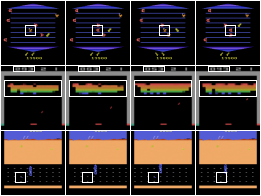
\includegraphics[width=\linewidth]{images/figure__iris_vs_diamond__iris.png}
    \caption{\textsc{iris}} \label{fig:iris_vs_diamond__iris}
  \end{subfigure}%
  \hspace*{\fill}   % maximize separation between the subfigures
  \begin{subfigure}{0.49\textwidth}
    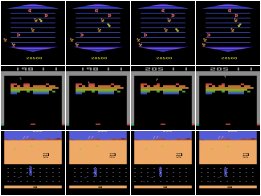
\includegraphics[width=\linewidth]{images/figure__iris_vs_diamond__diamond.png}
    \caption{\textsc{diamond}} \label{fig:iris_vs_diamond__diamond}
  \end{subfigure}%
\caption{Consecutive frames imagined with \textsc{iris} (left) and \textsc{diamond} (right). The white boxes highlight inconsistencies between frames, which we see only arise in trajectories generated with \textsc{iris}. In \textit{Asterix} (top row), an enemy (orange) becomes a reward (red) in the second frame, before reverting to an enemy in the third, and again to a reward in the fourth. In \textit{Breakout} (middle row), the bricks and score are inconsistent between frames. In \textit{Road Runner} (bottom row), the rewards (small blue dots on the road) are inconsistently rendered between frames. None of these inconsistencies occur with \textsc{diamond}. In \textit{Breakout}, the score is even reliably updated by +7 when a red brick is broken\protect\footnotemark.}
\label{fig:iris_vs_diamond}
\end{figure}

\footnotetext{\href{https://en.wikipedia.org/wiki/Breakout_(video_game)\#Gameplay}{\texttt{https://en.wikipedia.org/wiki/Breakout\_(video\_game)\#Gameplay}}}
% %%%%%%%%%%%%%%%%%%%%%%%

We see in Figure \ref{fig:iris_vs_diamond} that the trajectories imagined by \textsc{diamond} are generally of higher visual quality and more faithful to the true environment compared to the trajectories imagined by \textsc{iris}. In particular, the trajectories generated by \textsc{iris} contain visual inconsistencies between frames (highlighted by white boxes), such as enemies being displayed as rewards and vice-versa. These inconsistencies may only represent a few pixels in the generated images, but can have significant consequences for reinforcement learning. For example, since an agent should generally target rewards and avoid enemies, these small visual discrepancies can make it more challenging to learn an optimal policy.

These improvements in the consistency of visual details are generally reflected by greater agent performance on these games, as shown in Table \ref{tab:atari_results_full}. Since the agent component of these methods is similar, this improvement can likely be attributed to the world model. 

Finally, we note that this improvement is not simply the result of increased computation. Both world models are rendering frames at the same resolution ($64\times64$), and \textsc{diamond} requires only 3 NFE per frame compared to 16 NFE per frame for \textsc{iris}. This is further reflected by the fact that \textsc{diamond} has significantly fewer parameters and takes less time to train than \textsc{iris}, as provided in Appendix \ref{app:performance_profile}.
\section{Scaling the diffusion world model to \textit{Counter-Strike: Global Offensive}\protect\footnote{This section was added after NeurIPS acceptance, following community interest in later CS:GO experiments.}}
\label{sec:csgo}

To investigate the ability of \textsc{diamond}'s diffusion world model to learn to model more complex 3D environments, we train the world model in isolation on static data from the popular video game \textit{Counter-Strike: Global Offensive} (CS:GO). We use the \textit{Online} dataset of 5.5M frames (95 hours) of online human gameplay captured at 16Hz from the map \textit{Dust II} by \citet{pearce2022counter}. We randomly hold out 0.5M frames (corresponding to 500 episodes, or 8 hours) for testing, and use the remaining 5M frames (87 hours) for training. There is no reinforcement learning agent or online data collection involved in these experiments.

To reduce the computational cost, we reduce the resolution from $(280\times150)$ to $(56\times30)$ for world modeling. We then introduce a second, smaller diffusion model as an upsampler to improve the generated images at the original resolution \citep{saharia2022image}. We scale the channels of the U-Net to increase the number of parameters from 4M for our Atari models to 381M for our CS:GO model (including 51M for the upsampler). The combined model was trained for 12 days on an RTX 4090. 

Finally, we introduce stochastic sampling and increase the number of denoising steps for the upsampler to 10, which we found to improve the resulting visual quality of the generations, while keeping the dynamics model the same (in particular, still using only 3 denoising steps). This enables a reasonable tradeoff between visual quality and inference cost, with the model running at 10Hz on an RTX 3090. Typical generations of the model are provided in Figure \ref{fig:csgo_grid} below.

%%%%%%%%%%%%%%%%%%%%%%%
\begin{figure}[h]
%\vspace{-6mm}
\begin{center}
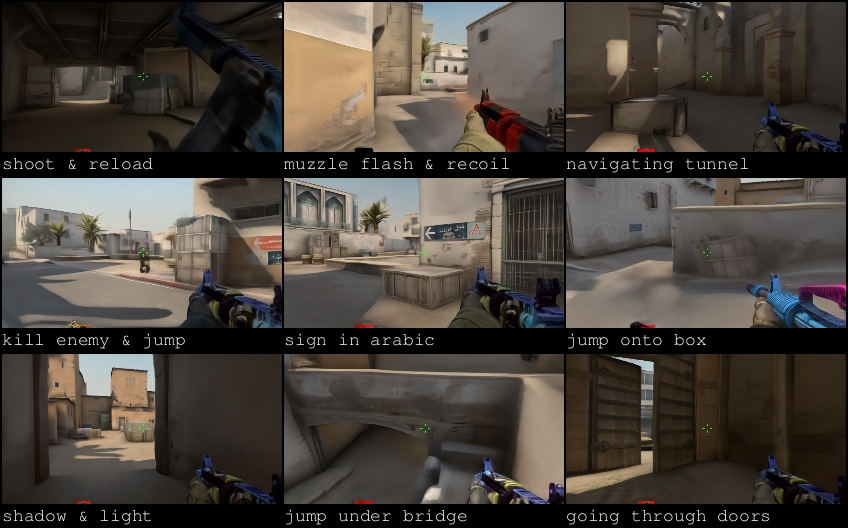
\includegraphics[width=.7\linewidth]{images/csgo_grid.png}
\caption{Images captured from people playing with keyboard and mouse inside \textsc{diamond}'s diffusion world model. This model was trained on $87$ hours of static \textit{Counter-Strike: Global Offensive} (CS:GO) gameplay \citep{pearce2022counter} to produce an interactive neural game engine for the popular in-game map, \textit{Dust II}. Best viewed as videos at \wslink.}
\label{fig:csgo_grid}
\end{center}
\vspace{-4mm}
\end{figure}
%%%%%%%%%%%%%%%%%%%%%%%

We find the model is able to generate stable trajectories over hundreds of timesteps, although is more likely to drift out-of-distribution in less frequently visited areas of the map. Due to the limited memory of the model, approaching walls or losing visibility may cause the model to forget the current state and instead generate a new weapon or area of map. Interestingly, we find the model wrongly enables successive jumps by generalizing the effect of a jump on the geometry of the scene, since multiple jumps do not appear often enough in the training gameplay for the model to learn that mid-air jumps should be ignored. We expect scaling the model and data to address many of these limitations, with the exception of the memory of the model. Quantitative measurements of the capabilities of the CS:GO world model and attempts to address these limitations are left to future work.

% %%%%%%%%%%%%%%%%%%%%%%%
% \begin{wrapfigure}[]{R}{0.55\linewidth}
% \vspace{-5mm}
% \begin{center}
% \centerline{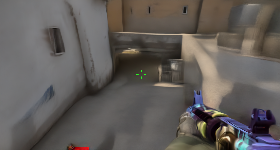
\includegraphics[width=\linewidth]{images/csgo_jump.png}}
% \caption{Looking down at the map after multiple jumps. The model enables multiple jumps by generalizing the effect of a jump on the geometry of the scene, even though only a single jump should be possible. Full video available at \url{https://diamond-wm.github.io}.}
% \label{fig:csgo_jump}
% \end{center}
% \vskip 0in
% \end{wrapfigure}
% %%%%%%%%%%%%%%%%%%%%%%%



% \begin{itemize}
%     \item Motivation: Investigate application of diffusion world model to 3d environment as more complex
%     \item Figure: Example trajectories at different timesteps to show stability (and kb/mouse). Add link to video/website.
%     \item Method: No RL though, things we changed
%     \item Details: In order to reproduce - scaling UNet, discuss actions?, rect not square
%     \item Found stochastic sampling to help
%     \item Results: Playable at 10Hz, long stable trajectories if stay in distribution
%     \item Jump (claim 3d, but be cautious about reasons)
%     \item Limitations + Future work: scaling data/compute, CFG, proper measurements (App J)
% \end{itemize}

% \begin{itemize}
%     \item TODO: Add Generative Game Engine paragraph to related work.
%     \item TODO: update abstract to mention CSGO and website
%     \item TODO: update introduction/conclusion with csgo
%     \item TODO: Update previous CSGO appendix to 'early' experiments
%     \item TODO: Add rebuttal work (training times and DDPM drift) to appendix with mentions from main text
%     \item TODO: Check rebuttal for other promises
% \end{itemize}
\section{Related work}
\label{sec:related_work}

\textbf{World models.} The idea of reinforcement learning (RL) in the imagination of a neural network world model was introduced by \citet{ha2018world}. SimPLe \citep{kaiser2019atari100k} applied world models to Atari, and introduced the Atari 100k benchmark to focus on sample efficiency. Dreamer \citep{hafner2020dream} introduced RL from the latent space of a recurrent state space model (RSSM). DreamerV2 \citep{hafner2021mastering} demonstrated that using discrete latents could help to reduce compounding error, and DreamerV3 \citep{hafner2023dreamerv3} was able to achieve human-level performance on a wide range of domains with fixed hyperparameters. TWM \citep{robine2023transformer} adapts DreamerV2's RSSM to use a transformer architecture, while STORM \citep{zhang2023storm} adapts DreamerV3 in a similar way but with a different tokenization approach. Alternatively, IRIS \citep{iris2023} builds a language of image tokens with a discrete autoencoder, and composes these tokens over time with an autoregressive transformer. 

\textbf{Generative vision models.} There are parallels between these world models and image generation models which suggests that developments in generative vision models could provide benefits to world modeling. Following the rise of transformers in natural language processing \citep{vaswani2017attention,devlin2018bert,radford2019language}, VQGAN \citep{esser2021taming} and DALL·E \citep{ramesh2021zero} convert images to discrete tokens with discrete autoencoders \citep{vqvae}, and leverage the sequence modeling abilities of autoregressive transformers to build powerful text-to-image generative models. Concurrently, diffusion models \citep{sohl2015difforigin,ho2020DDPM,song_sde} gained traction \citep{dhariwal2021diffbeatsgans,ldm_stable_diffusion}, and have become a dominant paradigm for high-resolution image generation \citep{saharia2022imagen,ramesh2022hierarchical,podell2023sdxl}.

The same trends have taken place in the recent developments of video generation methods. VideoGPT \citep{yan2021videogpt} provides a minimal video generation architecture by combining a discrete autoencoder with an autoregressive transformer. Godiva \citep{wu2021godiva} enables text conditioning with promising generalization. Phenaki \citep{phenaki} allows arbitrary length video generation with sequential prompt conditioning. TECO \citep{yan2023teco} improves upon autoregressive modeling by using MaskGit \citep{chang2022maskgit}, and enables longer temporal dependencies by compressing input sequence embeddings. Diffusion models have also seen a resurgence in video generation using 3D U-Nets to provide high quality but short-duration video \citep{singer2023make,bar2024lumiere}. 
Recently, transformer-based diffusion models such as DiT  \citep{dit2023} and Sora \citep{sora2024} have shown improved scalability for both image and video generation, respectively.

\textbf{Diffusion for reinforcement learning.} There has also been much interest in combining diffusion models with reinforcement learning. This includes taking advantage of the flexibility of diffusion models as a policy \citep{wang2022diffusion, ajay2022conditional,pearce2023imitating}, as planners \citep{janner2022planning, liang2023adaptdiffuser}, as reward models \citep{nuti2023extracting}, and trajectory modeling for data augmentation in offline RL \citep{lu2023synthetic,ding2024diffusion,jackson2024policyguided}. \textsc{diamond} represents the first use of diffusion models as world models for learning online in imagination. 

\textbf{Generative game engines.} Playable games running entirely on neural networks have recently been growing in scope. \textit{GameGAN} \citep{gameGAN2020} learns generative models of games using a GAN \citep{goodfellow2014GAN} while \citet{bamford2020neural} use a Neural GPU \citep{kaiser2015neural}. Concurrent work includes \textit{Genie} \citep{bruce2024genie}, which generates playable platformer environments from image prompts, and \textit{GameNGen} \citep{valevski2024diffusionmodelsrealtimegame}, which similarly leverages a diffusion model to obtain a high resolution simulator of the game DOOM, but at a larger scale.
\vspace{-2mm}
\section{Limitations}
\label{sec:limitations}

We identify three main limitations of our work for future research. First, our main evaluation is focused on discrete control environments, and applying \textsc{diamond} to the continuous domain may provide additional insights. Second, the use of frame stacking for conditioning is a minimal mechanism to provide a memory of past observations. Integrating an autoregressive transformer over environment time, using an approach such as \citet{dit2023}, would enable longer-term memory and better scalability. We include an initial investigation into a potential cross-attention architecture in Appendix \ref{app:additonal_experiments}, but found frame-stacking more effective in our early experiments. Third, we leave potential integration of the reward/termination prediction into the diffusion model for future work, since combining these objectives and extracting representations from a diffusion model is not trivial \citep{luo2023dhf, xu2023open} and would make our world model unnecessarily complex.

\vspace{-2mm}
\section{Conclusion and Broader Impact}
\label{sec:conclusion}

We have introduced \textsc{diamond}, a reinforcement learning agent trained in a diffusion world model. 
We explained the key design choices we made to adapt diffusion for world modeling and to make our world model stable over long time horizons with a low number of denoising steps.
\textsc{diamond} achieves a mean human normalized score of $1.46$ on the well-established Atari 100k benchmark; a new best among agents trained entirely within a world model. 
We analyzed our improved performance in some games and found that it likely follows from better modeling of critical visual details.
We further demonstrated \textsc{diamond}'s diffusion world model can successfully model 3D environments and serve as a real-time neural game engine by training on static \textit{Counter-Strike: Global Offensive} gameplay.

World models constitute a promising direction to address sample efficiency and safety concerns associated with training agents in the real world. However, imperfections in the world model may lead to suboptimal or unexpected agent behaviors. We hope that the development of more faithful and interactive world models will contribute to broader efforts to further reduce these risks.

%The development of more visually faithful world models such as \textsc{diamond} provides a promising avenue to further reduce these risks.% associated with deploying agents trained in simulation. 

%hope that developing more visually faithful world models such as \textsc{diamond} constitutes a promising avenue to further reduce these risks. 

%In general, the deployment of agents in the real world raises safety concerns. Training in a world model reduces these risks by minimizing the time spent in the real environment, but imperfect world models may lead to unexpected agent behaviors. The development of more visually faithful world models such as \textsc{diamond} provides a promising avenue to further reduce the risks associated with deploying agents trained in simulation. 



%Our work considers the training of autonomous agents using a world model. 

%Taking a step back, the deployment of autonomous agents in the real world raises safety concerns regarding the potential harm they may cause, and training in a world model reduces these risks by minimizing the time the agent spends interacting with the environment. However, imperfect world models may lead to unexpected behaviors upon deployment of agents in the real-world, and the development of more realistic world models such as \textsc{diamond} provides a promising avenue to further reduce the risks associated with deploying agents trained in simulation.

%Additionally, as with all advances in the field of Machine Learning, there are many other potential societal consequences of our work, but none of which we feel must be specifically highlighted here.

% We have introduced \textsc{diamond}, a visually faithful diffusion world model for training agents in imagination. We explained key design choices for \textsc{diamond}'s diffusion world model that enables our implementation to remain stable over long time horizons with a low number of denoising steps. We demonstrate that this improved visual quality translates into improved agent performance on the well-established Atari 100k benchmark. As a result, \textsc{diamond} achieves a new state of the art among world model agents on this benchmark, with a mean human normalized score of $1.46$. The performance improvements are particularly evident for visually challenging environments, which is a promising sign that \textsc{diamond} could scale to visually complex real-world environments.
% % which is promising for scaling \textsc{diamond} to more visually complex real-world environments.

% This paper considers the training of autonomous agents using a world model. The deployment of autonomous agents in the real world raises safety concerns regarding the potential harm that may be caused by an agent's actions. Training in simulation reduces these risks by reducing the time the agent spends interacting with the environment. However, imperfect world models may lead to unexpected behaviors in the real world. The development of more realistic world models should therefore reduce the risk associated with deploying agents trained in this manner. Additionally, as with all advances in the field of Machine Learning, there are many other potential societal consequences of our work, but none of which we feel must be specifically highlighted here.

\newpage
 %\section*{Broader Impact}
% This paper considers the training of autonomous agents using a world model. The deployment of autonomous agents in the real world raises safety concerns regarding the potential harm that may be caused by an agent's actions. Training in simulation reduces these risks by reducing the time the agent spends interacting with the environment. However, imperfect world models may lead to unexpected behaviors in the real world. The development of more realistic world models should therefore reduce the risk associated with deploying agents trained in this manner. Additionally, as with all advances in the field of Machine Learning, there are many other potential societal consequences of our work, but none of which we feel must be specifically highlighted here.

\begin{ack}

We would like to thank Andrew Foong, Bálint Máté, Clément Vignac, Maxim Peter, Pedro Sanchez, Rich Turner, Stéphane Nguyen, Tom Lee, Trevor McInroe and Weipu Zhang for insightful discussions and comments.
Adam and Eloi met during an internship at Microsoft Research Cambridge, and would like to thank the Game Intelligence team, including Anssi Kanervisto, Dave Bignell, Gunshi Gupta, Katja Hofmann, Lukas Schäfer, Raluca Georgescu, Sam Devlin, Sergio Valcarcel Macua, Shanzheng Tan, Tabish Rashid, Tarun Gupta, Tim Pearce, and Yuhan Cao, for their support in the early stages of this project, and a great summer.

\end{ack}


\bibliography{main}
\bibliographystyle{apalike}


%%%%%%%%%%%%%%%%%%%%%%%%%%%%%%%%%%%%%%%%%%%%%%%%%%%%%%%%%%%%

\newpage
\appendix
\section{Sampling observations in \textsc{diamond}}
\label{appendix:sampling}

We describe here how we sample an observation $\x_t^0$ from our diffusion world model. We initialize the procedure with a noisy observation $\x_t^\Tau \sim p^{prior}$, and iteratively solve the reverse SDE in Equation \ref{eq:reverse_process} from $\tau = \Tau$ to $\tau = 0$, using the learned score model $\mathbf{S}_\theta(\x_t^\tau, \tau, \x_{<t}^0, a_{<t})$ conditioned on past observations $\x_{<t}^0$ and actions $a_{<t}$. This procedure is illustrated in Figure \ref{fig:architecture}.

In fact, there are many possible sampling methods for a given learned score model $\mathbf{S}_\theta$ \citep{karras2022elucidating}. Notably, \citet{song_sde} introduce a corresponding ``probability flow" ordinary differential equation (ODE), with marginals equivalent to the stochastic process described in Section \ref{subsec:diffusion}. In that case, the solving procedure is deterministic, and the only randomness comes from sampling the initial condition. In practice, this means that for a given score model, we can resort to any ODE or SDE solver, from simple first order methods like Euler (deterministic) and Euler–Maruyama (stochastic) schemes, to higher-order methods like Heun's method \citep{ascher1998computer}. 

Regardless of the choice of solver, each step introduces truncation errors, resulting from the local score approximation and the discretization of the continuous process. Higher order samplers may reduce this truncation error, but come at the cost of additional Number of Function Evaluations (NFE) -- how many forward passes of the network are required to generate a sample. This local error generally scales superlinearly with respect to the step size (for instance Euler's method is $\mathcal{O}(h^2)$ for step size $h$), so increasing the number of denoising steps improves the visual quality of the generated next frame. Therefore, there is a trade-off between visual quality and NFE that directly determines the inference cost of the diffusion world model.


% with t+1 instead of t

% \section{Sampling next observations in \textsc{diamond}}
% \label{appendix:sampling}

% We describe here how we sample a next observation $\x_{t+1}$ from our diffusion world model. We initialize the procedure with a noisy next observation $\x_{t+1}^\Tau \sim p^{prior}$, and iteratively solve the reverse SDE in Equation \ref{eq:reverse_process} from $\tau = \Tau$ to $\tau = 0$, using the learned score model $\mathbf{S}_\theta(\x_{t+1}^\tau, \tau, \x_{\le t}^0, a_{\le t})$ conditioned on past observations $\x_{\le t}^0$ and actions $a_{\le t}$. This procedure is illustrated in Figure \ref{fig:architecture}.

% In fact, there are many possible sampling methods for a given learned score model $S_\theta$ \citep{karras2022elucidating}. Notably, \citet{song_sde} introduce a corresponding ``probability flow" ordinary differential equation (ODE), with equivalent marginals. In that case, the solving procedure is deterministic, and the only randomness comes from sampling the initial condition. In practice, this means that for a given score model, we can resort to any ODE or SDE solver, from simple first order methods like Euler (deterministic) and Euler–Maruyama (stochastic) schemes, to higher-order methods like Heun's method \citep{ascher1998computer}. 

% Regardless of the choice of solver, each step introduces truncation errors, resulting from the local score approximation and the discretization of the continuous process. Higher order samplers may reduce this truncation error, but come at the cost of additional Number of Function Evaluations (NFE) -- how many forward passes of the network are required to generate a sample. This local error generally scales superlinearly with respect to the step size (for instance Euler's method is $\mathcal{O}(h^2)$ for step size $h$), so increasing the number of denoising steps improves the visual quality of the generated next frame. Therefore, there is a trade-off between visual quality and NFE that directly determines the inference cost of the diffusion world model.



\section{Link between DDPM and continuous-time score-based diffusion models}
\label{app:ddpm}

Denoising Diffusion Probabilistic Models (\textsc{ddpm}, \citet{ho2020DDPM}) can be described as a discrete version of the diffusion process introduced in Section \ref{subsec:diffusion}, as described in \citet{song_sde}. The discrete forward process is a Markov chain characterized by a discrete noise schedule $0 < \beta_1, \dots, \beta_i, \dots \beta_N < 1$, and a variance-preserving Gaussian transition kernel,

\begin{equation}
    p(\x^i|\x^{i-1}) = \mathcal{N}(\x^i; \sqrt{1-\beta_i} \x^{i-1}, \beta_i \mathbf{I}).
\end{equation}

In the continuous time limit $N \to \infty$, the Markov chain becomes a diffusion process, and the discrete noise schedule becomes a time-dependent function $\beta(\tau)$. This diffusion process can be described by an SDE with drift coefficient $\mathbf{f}(\x, \tau) = -\frac{1}{2}\beta(\tau)\x$ and diffusion coefficient $g(\tau) = \sqrt{\beta(\tau)}$ \citep{song_sde}. 


\section{\textsc{EDM} network preconditioners and training}
\label{appendix:karras_conditioners}

\citet{karras2022elucidating} use the following preconditioners for normalization and rescaling purposes (as mentioned in Section \ref{subsec:practical_dwm}) to improve network training:

\begin{equation}
    c_{in}^\tau = \frac{1}{\sqrt{\sigma(\tau)^2 + \sigma_{data}^2}}
\end{equation}
\begin{equation}
    c_{out}^\tau = \frac{\sigma(\tau)\sigma_{data}}{\sqrt{\sigma(\tau)^2 + \sigma_{data}^2}}
\end{equation}
\begin{equation}
    c_{noise}^\tau = \frac{1}{4}\log(\sigma(\tau))
\end{equation}
\begin{equation}
    c_{skip}^\tau = \frac{\sigma_{data}^2}{\sigma_{data}^2 + \sigma^2(\tau)},
\end{equation}
where $\sigma_{data}=0.5$.

The noise parameter $\sigma(\tau)$ is sampled to maximize the effectiveness of training as follows:
\begin{equation}
\log(\sigma(\tau))\sim \mathcal{N}(P_{mean}, P_{std}^2),
\end{equation}
where $P_{mean}=-0.4, P_{std}=1.2$. Refer to \citet{karras2022elucidating} for an in-depth analysis.
\newpage
\section{Model architectures}\label{app:architectures}

The diffusion model $\mathbf{D}_\theta$ is a standard U-Net 2D \citep{ronneberger2015unet}, conditioned on the last 4 frames and actions, as well as the diffusion time $\tau$. We use frame stacking for observation conditioning, and adaptive group normalization \citep{adagn} for action and diffusion time conditioning.

The reward/termination model $R_\psi$ layers are shared except for the final prediction heads. The model takes as input a sequence of frames and actions, and forwards it through convolutional residual blocks \citep{He2015} followed by an LSTM cell \citep{a3c,lstm,Gers2000}. Before starting the imagination procedure, we burn-in \citep{r2d2} the conditioning frames and actions to initialize the hidden and cell states of the LSTM. 

The weights of the policy $\pi_\phi$ and value network $V_\phi$ are shared except for the last layer. In the following, we refer to $(\pi,V)_\phi$ as the "actor-critic" network, even though $V$ is technically a state-value network, not a critic. This network takes as input a frame, and forwards it through convolutional trunk followed by an LSTM cell. The convolutional trunk consists of four residual blocks and 2x2 max-pooling with stride 2. The main path of the residual blocks consists of a group normalization \citep{groupnorm} layer, a SiLU activation \citep{elfwing2018sigmoid}, and a 3x3 convolution with stride 1 and padding 1. Before starting the imagination procedure, we burn-in the conditioning frames to initialize the hidden and cell states of the LSTM. 


Please refer to Table \ref{tbl_architecture} below for hyperparameter values, and to Algorithm \ref{alg:diamond} for a detailed summary of the training procedure. 

\vspace{1cm}

\begin{table}[h!]
\caption{Architecture details for \textsc{diamond}.}
\label{tbl_architecture}
\begin{center}
% \resizebox{0.4 \columnwidth}{!}{
\begin{tabular}{ l c }
\multicolumn{1}{c}{\textbf{Hyperparameter}}  & \multicolumn{1}{c}{\textbf{Value}} \\ 

\hline \\

% \hline \\
\\
\multicolumn{2}{l}{\textbf{Diffusion Model ($\mathbf{D}_\theta$)}} \\
% Number of conditioning observations/actions ($L$) & 4 \\
Observation conditioning mechanism & Frame stacking \\
Action conditioning mechanism & Adaptive Group Normalization \\
Diffusion time conditioning mechanism & Adaptive Group Normalization \\
Residual blocks layers & [2, 2, 2, 2] \\
Residual blocks channels & [64, 64, 64, 64] \\
Residual blocks conditioning dimension & 256 \\

% \hline \\
\\
\multicolumn{2}{l}{\textbf{Reward/Termination Model ($R_\psi$)}} \\
Action conditioning mechanisms & Adaptive Group Normalization \\
Residual blocks layers & [2, 2, 2, 2] \\
Residual blocks channels & [32, 32, 32, 32] \\
Residual blocks conditioning dimension & 128 \\
LSTM dimension & 512 \\ 
% Burn-in length ($B_{rt}$), set as $B_{rt} = L$ in practice & 4 \\ 
% Training sequence length ($B_{rt} + H$) & 19 \\

% \hline \\
\\
\multicolumn{2}{l}{\textbf{Actor-Critic Model ($\pi_\phi$ and $V_\phi$)}} \\
Residual blocks layers & [1, 1, 1, 1] \\
Residual blocks channels & [32, 32, 64, 64] \\
LSTM dimension & 512 \\ 
% Burn-in length ($B_{ac}$), set as $B_{ac} = L$ in practice & 4 \\


\end{tabular}
% }
\end{center}
\end{table}

\newpage
\begin{tabular}{@{}l|ccccc@{}}
\toprule
 & \multicolumn{5}{c}{PoolFormer} \\ 
 & S12 & S24 & S36 & M36 & M48 \\
\midrule
Peak drop rate of stoch. depth $d_r$ & 0.1 & 0.1 & 0.2 & 0.3 & 0.4 \\
LayerScale initialization $\epsilon$ & $10^{-5}$ & $10^{-5}$ & $10^{-6}$ & $10^{-6}$ & $10^{-6}$ \\
\hline
Data augmentation & \multicolumn{5}{c}{AutoAugment} \\
Repeated Augmentation & \multicolumn{5}{c}{off} \\
Input resolution & \multicolumn{5}{c}{224} \\
Epochs & \multicolumn{5}{c}{300} \\
Warmup epochs & \multicolumn{5}{c}{5} \\
Hidden dropout & \multicolumn{5}{c}{0} \\
GeLU dropout & \multicolumn{5}{c}{0} \\
Classification dropout & \multicolumn{5}{c}{0} \\
Random erasing prob & \multicolumn{5}{c}{0.25} \\
EMA decay & \multicolumn{5}{c}{0} \\
Cutmix $\alpha$ & \multicolumn{5}{c}{1.0} \\
Mixup $\alpha$ & \multicolumn{5}{c}{0.8} \\
Cutmix-Mixup switch prob & \multicolumn{5}{c}{0.5} \\
Label smoothing & \multicolumn{5}{c}{0.1} \\
\tabincell{l}{Relation between peak learning \\ \qquad rate and batch size} & \multicolumn{5}{c}{$\mathrm{lr} = \frac{\mathrm{batch\_size}}{1024}\times 10^{-3}$} \\
Batch size used in the paper & \multicolumn{5}{c}{4096} \\
Peak learning rate used in the paper & \multicolumn{5}{c}{$4 \times 10^{-4}$} \\
Learning rate decay & \multicolumn{5}{c}{cosine} \\
Optimizer & \multicolumn{5}{c}{AdamW} \\
Adam $\epsilon$ & \multicolumn{5}{c}{1e-8} \\
Adam $(\beta_1, \beta_2)$ & \multicolumn{5}{c}{(0.9, 0.999)} \\
Weight decay & \multicolumn{5}{c}{0.05} \\
Gradient clipping & \multicolumn{5}{c}{None} \\
\bottomrule
\end{tabular}
\newpage
\section{Reinforcement learning objectives}
\label{appendix:rl_actor_critic}

In what follows, we note $\x_t$, $r_t$ and $d_t$ the observations, rewards, and boolean episode terminations predicted by our world model. We note $H$ the imagination horizon, $V_\phi$ the value network, $\pi_\phi$ the policy network, and $a_t$ the actions taken by the policy within the world model. 

We use $\lambda$-returns to balance bias and variance as the regression target for the value network. Given an imagined trajectory of length $H$, we can define the $\lambda$-return recursively as follows,

\begin{equation}
\Lambda_t = 
\begin{cases}
    r_t + \gamma (1 - d_t) \Big[ (1 - \lambda) V_\phi(\x_{t+1}) + \lambda \Lambda_{t+1} \Big]   & \text{if}\quad t < H \\
    V_\phi(\x_H)                                                                                            & \text{if}\quad t = H. \\
\end{cases}
\end{equation}

The value network $V_\phi$ is trained to minimize $\mathcal{L}_V(\phi)$, the expected squared difference with $\lambda$-returns over imagined trajectories,

\begin{equation}
\mathcal{L}_V(\phi) = \mathbb{E}_{\pi_\phi} \left[ \sum_{t=0}^{H-1} \big( V_\phi(\x_t) - \mathrm{sg} ( \Lambda_t ) \big)^2 \right],
\end{equation}

where $\operatorname{sg}(\cdot)$ denotes the gradient stopping operation, meaning that the target is a constant in the gradient-based optimization, as classically established in the literature \citep{mnih2015dqn,hafner2021mastering,iris2023}.

As we can generate large amounts of on-policy trajectories in imagination, we use a simple \textsc{reinforce} objective to train the policy, with the value $V_\phi(\x_t)$ as a baseline to reduce the variance of the gradients \citep{sutton2018reinforcement}. The policy is trained to minimize the following objective, combining \textsc{reinforce} and a weighted entropy maximization objective to maintain sufficient exploration,

\begin{equation}
\mathcal{L}_\pi(\phi) = - \mathbb{E}_{\pi_\phi} \left[ \sum_{t=0}^{H-1} \log\left(\pi_\phi\left(a_t \mid \x_{\le t}\right)\right) \operatorname{sg}\left(\Lambda_t - V_\phi\left(\x_t\right)\right) + \eta \operatorname{\mathcal{H}}\left(\pi_\phi \left(a_t \mid \x_{\le t} \right) \right)\right].
\end{equation}

\vspace{1cm}


\newpage
% ALGORITHM STYLE -- Released 8 April 1996
%    for LaTeX-2e
% Copyright -- 1994 Peter Williams
% E-mail Peter.Williams@dsto.defence.gov.au
\NeedsTeXFormat{LaTeX2e}
\ProvidesPackage{algorithm}
\typeout{Document Style `algorithm' - floating environment}

\RequirePackage{float}
\RequirePackage{ifthen}
\newcommand{\ALG@within}{nothing}
\newboolean{ALG@within}
\setboolean{ALG@within}{false}
\newcommand{\ALG@floatstyle}{ruled}
\newcommand{\ALG@name}{Algorithm}
\newcommand{\listalgorithmname}{List of \ALG@name s}

% Declare Options
% first appearance
\DeclareOption{plain}{
  \renewcommand{\ALG@floatstyle}{plain}
}
\DeclareOption{ruled}{
  \renewcommand{\ALG@floatstyle}{ruled}
}
\DeclareOption{boxed}{
  \renewcommand{\ALG@floatstyle}{boxed}
}
% then numbering convention
\DeclareOption{part}{
  \renewcommand{\ALG@within}{part}
  \setboolean{ALG@within}{true}
}
\DeclareOption{chapter}{
  \renewcommand{\ALG@within}{chapter}
  \setboolean{ALG@within}{true}
}
\DeclareOption{section}{
  \renewcommand{\ALG@within}{section}
  \setboolean{ALG@within}{true}
}
\DeclareOption{subsection}{
  \renewcommand{\ALG@within}{subsection}
  \setboolean{ALG@within}{true}
}
\DeclareOption{subsubsection}{
  \renewcommand{\ALG@within}{subsubsection}
  \setboolean{ALG@within}{true}
}
\DeclareOption{nothing}{
  \renewcommand{\ALG@within}{nothing}
  \setboolean{ALG@within}{true}
}
\DeclareOption*{\edef\ALG@name{\CurrentOption}}

% ALGORITHM
%
\ProcessOptions
\floatstyle{\ALG@floatstyle}
\ifthenelse{\boolean{ALG@within}}{
  \ifthenelse{\equal{\ALG@within}{part}}
     {\newfloat{algorithm}{htbp}{loa}[part]}{}
  \ifthenelse{\equal{\ALG@within}{chapter}}
     {\newfloat{algorithm}{htbp}{loa}[chapter]}{}
  \ifthenelse{\equal{\ALG@within}{section}}
     {\newfloat{algorithm}{htbp}{loa}[section]}{}
  \ifthenelse{\equal{\ALG@within}{subsection}}
     {\newfloat{algorithm}{htbp}{loa}[subsection]}{}
  \ifthenelse{\equal{\ALG@within}{subsubsection}}
     {\newfloat{algorithm}{htbp}{loa}[subsubsection]}{}
  \ifthenelse{\equal{\ALG@within}{nothing}}
     {\newfloat{algorithm}{htbp}{loa}}{}
}{
  \newfloat{algorithm}{htbp}{loa}
}
\floatname{algorithm}{\ALG@name}

\newcommand{\listofalgorithms}{\listof{algorithm}{\listalgorithmname}}

\newpage
\section{Additional performance comparisons}
\label{app:performance_profile}

We provide performance profiles \citep{agarwal2021deep} for \textsc{diamond} and baselines below. % We see that \textsc{diamond} outperforms the baselines in terms of the fraction of runs above a given human normalized score for a range of scores.

%%%%%%%%%%%%%%%%%%%%%%%
\begin{figure}[h!]
\vskip 0.2in
\begin{center}
\centerline{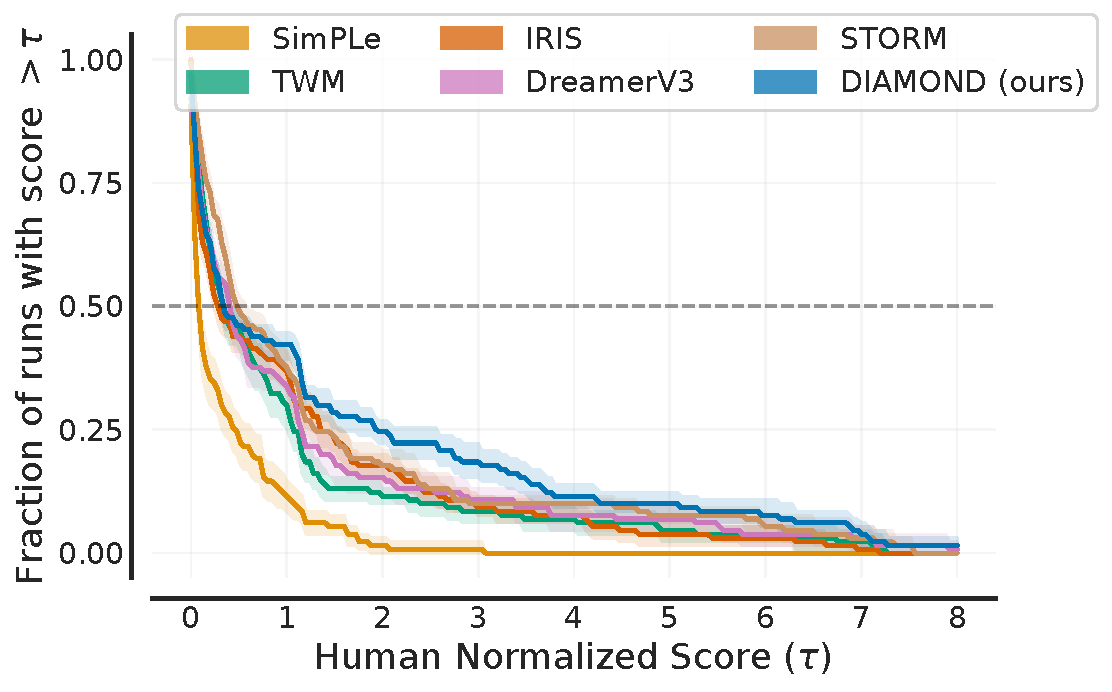
\includegraphics[width=.7\columnwidth]{images/performance_profile.pdf}}
\caption{Performance profiles, i.e. fraction of runs above a given human normalized score.}
\label{fig:results_performance_profile}
\end{center}
\vskip 0.2in
\end{figure}
%%%%%%%%%%%%%%%%%%%%%%%

As additional angles of comparison, we also provide parameter counts and approximate training times for \textsc{iris}, DreamerV3 and \textsc{diamond} in Table \ref{tab:training_time} below. We see that \textsc{diamond} has the highest mean HNS, with fewer parameters than both \textsc{iris} and DreamerV3. \textsc{diamond} also trains faster than \textsc{iris}, although is slower than DreamerV3. 

\begin{table}[h]
\caption{Number of parameters, training time, and mean human-normalized score (HNS).}
\label{tab:training_time}
\begin{center}
\begin{tabular}{lcccc}
\hline
    & \textsc{iris} & DreamerV3 & \textsc{diamond} (ours) & \\ \hline
\#parameters (↓)        & 30M       & 18M            & \textbf{13M}   &  \\
Training days (↓) & 4.1       & \textbf{\textless 1}   & 2.9   &  \\
Mean HNS (↑)            & 1.046     & 1.097          & \textbf{1.459} &  \\ \hline
\end{tabular}
\end{center}
\end{table}



A full training time profile for \textsc{diamond} is provided in Appendix~\ref{app:profiling}.
\newpage
\section{Training time profile}\label{app:profiling}

Table~\ref{tab:profiling} provides a full training time profile for \textsc{diamond}.

\begin{table}[h!]
\caption{Detailed breakdown of training time. Profiling performed using a Nvidia RTX 4090 with the default hyperparameters specified in Appendices \ref{app:architectures} and \ref{app:hyperparams} These profiling measures are representative, since exact durations will depend on the machine, the environment, and the training stage.}
\label{tab:profiling}
\begin{center}

\scalebox{1.0}{

\begin{tabular}{|>{\raggedright\arraybackslash}p{7cm}|>{\raggedleft\arraybackslash}p{2cm}|>{\raggedleft\arraybackslash}p{3.5cm}|}
    \hline
    \textbf{Single update} & \textbf{Time (ms)} & \textbf{Detail (ms)} \\
    \hline
    Total & $543$ & $88 + 115 + 340$\\
    \hspace{0.5cm} Diffusion model update & $88$ & - \\
    \hspace{0.5cm} Reward/Termination model update & $115$ & - \\
    \hspace{0.5cm} Actor-Critic model update & $340$ & $15 \times 20.4 + 34$\\
    \hspace{1cm} Imagination step (x 15) & $20.4$ & $12.7 + 7.0 + 0.7$ \\
    \hspace{1.5cm} Next observation prediction & $12.7$ & $3 \times 4.2$ \\
    \hspace{2cm} Denoising step (x 3) & $4.2$ & - \\
    \hspace{1.5cm} Reward/Termination prediction & $7.0$ & - \\
    \hspace{1.5cm} Action prediction & $0.7$ & - \\
    \hspace{1cm} Loss computation and backward & $34$ & - \\
    \hline
    \textbf{Epoch} & \textbf{Time (s)} & \textbf{Detail (s)} \\
    \hline
    Total & $217$ & $35 + 46 + 136$ \\
    \hspace{0.5cm} Diffusion model & $35$ & $400 \times 88 \times  10^{-3}$ \\
    \hspace{0.5cm} Reward/Termination model & $46$ & $400 \times 115 \times  10^{-3}$ \\
    \hspace{0.5cm} Actor-Critic model & $136$ & $400 \times 340 \times  10^{-3}$ \\
    \hline
    \textbf{Run} & \textbf{Time (days)} & \textbf{Detail (days)} \\
    \hline
    Total & $2.9$ & $2.5 + 0.4$ \\
    \hspace{0.5cm} Training time & $2.5$ & $1000 \times 217 / (24 \times 3600)$ \\
    \hspace{0.5cm} Other (collection, evaluation, checkpointing) & $0.4$ & - \\
    \hline
\end{tabular}

}

\end{center}
\end{table}
\label{tab:r}
%% \section{Scope and limitations}
% We frame many existing algorithms for composing models in terms of probabilistic programming. While this suggests the possibility of applying a variety of existing inference and train-time techniques to the resulting models, the present work does not evaluate methods beyond rejection sampling.
% 
% A challenge applying cascades in practice is the difficulty of probabilistic inference in models with string-valued variables. Previous work in particle based inference for probabilistic programs provides some hope in this direction \citep{anglican}.

% This perspective opens up exciting new directions in applications of language models, and in foundation models more generally.
% Existing fine-tuning methods can be described with a principled probabilistic programming language formalism representing structured distributions known as LM Cascades. This defines the distribution on the string-valued output of a large language model, the compositions of which may be adapted as specific inference algorithms underpinning various applications. 


% efficiency / expense
% We don't actually explore specific inference methods
% Hint of 
% hints @ lots of possibilities, explores very few of them
% - multimodality
% - train/test time inference beyond rejection sampling
% - tool use
\newpage
\section{Broader comparison to model-free and search-based methods}
\label{app:additonal_baselines}

Table \ref{tab:atari_results_other_baselines} provides scores for model-free and search-based methods, including the current best performing methods on the Atari 100k benchmark, EfficientZero \citep{ye2021efficientzero} and \textsc{bbf} \citep{schwarzer2023bigger}. Both of these methods use approaches that are out of scope of our approach, such as computationally expensive lookahead Monte-Carlo tree search for EfficientZero, and using periodic network resets in combination with hyperparameter scheduling for \textsc{bbf}. We see that while the use of lookahead search and more advanced reinforcement learning techniques (for EfficientZero \citep{ye2021efficientzero} and \textsc{bbf} \citep{schwarzer2023bigger} respectively) can still provide greater performance overall, \textsc{diamond} promisingly still outperforms these methods on some games.

\begin{table*}[h]
    \caption{Raw scores and human-normalized metrics for search-based and model-free methods.}
    \label{tab:atari_results_other_baselines}
\begin{center}
\begin{small}
\centering
\scalebox{0.86}{
\centering

\begin{tabular}{lrr rrrrrr}
\toprule
\multicolumn{2}{c}{} & \multicolumn{2}{c}{Search-based} & \multicolumn{4}{c}{Model-free} \\
\cmidrule(lr){3-4} \cmidrule(lr){5-8}
%%%%%%%%%%%%%%%%%%%%%%%%%%%%%%%%%%%%%%%%%%%%%%%%%%%%%%%%%%%%%%%%%%%%
Game                 &  Human     &  MuZero    &  EfficientZero      &  CURL     &  SPR       &  SR-SPR              &  BBF                &  \textsc{diamond} (ours)  \\
\midrule
Alien                &  7127.7    &  530.0     &  808.5              &  711.0    &  841.9     &  1107.8              &  \textbf{1173.2}    &  744.1                    \\
Amidar               &  1719.5    &  38.8      &  148.6              &  113.7    &  179.7     &  203.4               &  \textbf{244.6}     &  225.8                    \\
Assault              &  742.0     &  500.1     &  1263.1             &  500.9    &  565.6     &  1088.9              &  \textbf{2098.5}    &  1526.4                   \\
Asterix              &  8503.3    &  1734.0    &  \textbf{25557.8}   &  567.2    &  962.5     &  903.1               &  3946.1             &  3698.5                   \\
BankHeist            &  753.1     &  192.5     &  351.0              &  65.3     &  345.4     &  531.7               &  \textbf{732.9}     &  19.7                     \\
BattleZone           &  37187.5   &  7687.5    &  13871.2            &  8997.8   &  14834.1   &  17671.0             &  \textbf{24459.8}   &  4702.0                   \\
Boxing               &  12.1      &  15.1      &  52.7               &  0.9      &  35.7      &  45.8                &  85.8               &  \textbf{86.9}            \\
Breakout             &  30.5      &  48.0      &  \textbf{414.1}     &  2.6      &  19.6      &  25.5                &  370.6              &  132.5                    \\
ChopperCommand       &  7387.8    &  1350.0    &  1117.3             &  783.5    &  946.3     &  2362.1              &  \textbf{7549.3}    &  1369.8                   \\
CrazyClimber         &  35829.4   &  56937.0   &  83940.2            &  9154.4   &  36700.5   &  45544.1             &  58431.8            &  \textbf{99167.8}         \\
DemonAttack          &  1971.0    &  3527.0    &  13003.9            &  646.5    &  517.6     &  2814.4              &  \textbf{13341.4}   &  288.1                    \\
Freeway              &  29.6      &  21.8      &  21.8               &  28.3     &  19.3      &  25.4                &  25.5               &  \textbf{33.3}            \\
Frostbite            &  4334.7    &  255.0     &  296.3              &  1226.5   &  1170.7    &  \textbf{2584.8}     &  2384.8             &  274.1                    \\
Gopher               &  2412.5    &  1256.0    &  3260.3             &  400.9    &  660.6     &  712.4               &  1331.2             &  \textbf{5897.9}          \\
Hero                 &  30826.4   &  3095.0    &  \textbf{9315.9}    &  4987.7   &  5858.6    &  8524.0              &  7818.6             &  5621.8                   \\
Jamesbond            &  302.8     &  87.5      &  517.0              &  331.0    &  366.5     &  389.1               &  \textbf{1129.6}    &  427.4                    \\
Kangaroo             &  3035.0    &  62.5      &  724.1              &  740.2    &  3617.4    &  3631.7              &  \textbf{6614.7}    &  5382.2                   \\
Krull                &  2665.5    &  4890.8    &  5663.3             &  3049.2   &  3681.6    &  5911.8              &  8223.4             &  \textbf{8610.1}          \\
KungFuMaster         &  22736.3   &  18813.0   &  \textbf{30944.8}   &  8155.6   &  14783.2   &  18649.4             &  18991.7            &  18713.6                  \\
MsPacman             &  6951.6    &  1265.6    &  1281.2             &  1064.0   &  1318.4    &  1574.1              &  \textbf{2008.3}    &  1958.2                   \\
Pong                 &  14.6      &  -6.7      &  20.1               &  -18.5    &  -5.4      &  2.9                 &  16.7               &  \textbf{20.4}            \\
PrivateEye           &  69571.3   &  56.3      &  96.7               &  81.9     &  86.0      &  97.9                &  40.5               &  \textbf{114.3}           \\
Qbert                &  13455.0   &  3952.0    &  \textbf{13781.9}   &  727.0    &  866.3     &  4044.1              &  4447.1             &  4499.3                   \\
RoadRunner           &  7845.0    &  2500.0    &  17751.3            &  5006.1   &  12213.1   &  13463.4             &  \textbf{33426.8}   &  20673.2                  \\
Seaquest             &  42054.7   &  208.0     &  1100.2             &  315.2    &  558.1     &  819.0               &  \textbf{1232.5}    &  551.2                    \\
UpNDown              &  11693.2   &  2896.9    &  17264.2            &  2646.4   &  10859.2   &  \textbf{112450.3}   &  12101.7            &  3856.3                   \\
\midrule
\#Superhuman (↑)     &  N/A       &  5         &  \textbf{14}        &  2        &  6         &  9                   &  12                 &  11                       \\
Mean (↑)             &  1.000     &  0.562     &  1.943              &  0.261    &  0.616     &  1.271               &  \textbf{2.247}     &  1.459                    \\
IQM (↑)              &  1.000     &  0.288     &  1.047              &  0.113    &  0.337     &  0.700               &  \textbf{1.139}     &  0.641                    \\
%%%%%%%%%%%%%%%%%%%%%%%%%%%%%%%%%%%%%%%%%%%%%%%%%%%%%%%%%%%%%%%%%%

\bottomrule
\end{tabular}
 }
\end{small}
\end{center}
%\vspace{-0.02\linewidth}
\end{table*}

\newpage
\section{Quantitative analysis of autoregressive model drift}\label{app:ddpm_drift}

Figure~\ref{fig:ddpm_drift} provides a quantitative measure of the compounding error demonstrated qualitatively in Figure~\ref{fig:denoising_trajectories} for DDPM and EDM based world models.

\begin{figure}[h!]
\begin{center}
\centerline{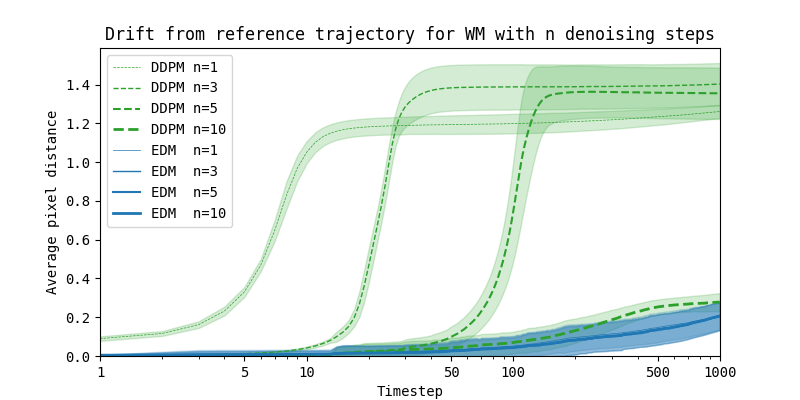
\includegraphics[width=\columnwidth]{images/drift.png}}
\caption{Average pixel drift between an imagined trajectory and the corresponding reference trajectory collected with an expert in \textit{Breakout}. The trajectories are each 1000 timesteps, starting from the same frame and following the same sequence of actions. Each line displays the average and shaded standard deviation of 400 reference trajectories held out from training data. DDPM becomes more stable with increasing number of denoising steps, but is less stable than 1-step EDM, even with 10 denoising steps. The drift we observe for EDM corresponds to differences in the imagined trajectory rather than a pathological color shift as we see in Figure 3a.}
\label{fig:ddpm_drift}
\end{center}
\end{figure}
\section{Quantitative ablation on reducing the number of denoising steps}\label{app:denoising_ablation}

Table~\ref{tab:ablation_rl_1_step} provides a quantitative ablation of the effect of reducing the number of denoising steps used for our EDM diffusion world model from 3 (used for Table~\ref{tab:atari_results_full}) to 1, for \textsc{diamond}'s 10 highest performing games. Note that the 1-step results correspond to a single seed only so will have higher variance. Nonetheless, these results provide some signal that agents trained with 1 denoising step perform worse than our default choice of 3, particularly for the game \textit{Boxing}, despite the apparent similarity in Figure~\ref{fig:ddpm_drift}. This additional evidence supports our qualitative analysis in Section \ref{subsec:denoising_steps}.

\begin{table*}[h]
\caption{Quantitative ablation on reducing the number of denoising steps from 3 (default) to 1.}
\label{tab:ablation_rl_1_step}
\begin{center}
\begin{small}
\centering
\scalebox{1.0}{
\centering
\begin{tabular}{lrr rr}
\toprule
%\multicolumn{3}{c}{} & \multicolumn{2}{c}{Model-free} & \multicolumn{5}{c}{Imagination-based} \\
%\cmidrule(lr){4-5} \cmidrule(lr){6-11}

%%%%%%%%%%%%%%%%%%%%%%%%%%%%%%%%%%%%%%%%%%%%%%%%%%%%%%%%%%%%%%%%%%%%
Game                 &  Random    &  Human     &  \textsc{diamond} ($n=3$)  & \textsc{diamond} ($n=1$)  \\
\midrule
Amidar               &  5.8       &  1719.5    &  \textbf{225.8}           & 191.8 \\
Assault              &  222.4     &  742.0     &  \textbf{1526.4}          & 782.5 \\
Asterix              &  210.0     &  8503.3    &          3698.5           & \textbf{6687.0} \\
Boxing               &  0.1       &  12.1      &  \textbf{86.9}            & 41.9            \\
Breakout             &  1.7       &  30.5      &  \textbf{132.5}           & 50.8            \\
CrazyClimber         &  10780.5   &  35829.4   &  \textbf{99167.8}         & 87233.0         \\
Kangaroo             &  52.0      &  3035.0    &  \textbf{5382.2}          & 1710.0          \\
Krull                &  1598.0    &  2665.5    &          8610.1           & \textbf{9105.1} \\
Pong                 &  -20.7     &  14.6      &          20.4             & \textbf{20.9}   \\
RoadRunner           &  11.5      &  7845.0    &  \textbf{20673.2}         & 5084.0          \\
\midrule
Mean HNS (↑)         &  0.000     &  1.000     &  \textbf{3.052}           & 1.962           \\
%%%%%%%%%%%%%%%%%%%%%%%%%%%%%%%%%%%%%%%%%%%%%%%%%%%%%%%%%%%%%%%%%%

\bottomrule
\end{tabular}
 }
\end{small}
\end{center}
%\vspace{-1cm}
\end{table*}
\newpage
% \section{Data Diversity Leads to Generalization}
\label{sec:data_diversity}
Our experiments thus far have linked training stability to rule commitment. In this section, we will show that models can, in fact, stabilize without a systematic rule---if they memorize their training instead. Less diverse training data produces models that stabilize through memorization, whereas more diverse training data produces models that commit to systematic rules. Furthermore, mirroring our previous findings in data complexity, intermediate levels of data diversity lead to highly unstable runs even when all examples induce the same rule. 
\subsection{Measuring Data Diversity}
\label{sec:data_diveristy}

We define the diversity of a dataset according to the syntactic similarity between different examples. 
We measure a sentence pair's similarity by the tree-edit distance (TED) of their latent tree representations \citep{Chomsky2015-bg}. When two sentences share the same syntax tree, transforming one into the other requires only leaf-node (i.e., vocabulary) changes. For example, \textit{My unicorn entertains her tyrannosaurus}, and, \textit{Your zebra eats some apples}, have different vocabulary but identical syntax trees. We define a dataset's diversity as the number of unique syntactic trees it contains. Similar methods are used to measure diversity in both natural language \citep{Huang2023-ab, Gao2024-fi, Ramirez2022-mx} and code \citep{Song2024-cg}. 

\subsection{Diversity and stability}
\label{sec:inverse}

We will next show that when the model is exposed to fewer unique syntax trees during training, it memorizes their patterns without reliably applying rules to unseen structures. We demonstrate the effect by designing datasets to induce either hierarchical or linear generalization and then adjusting adjusting the syntactic diversity of representative examples. Whichever rule is induced, diversity imposes three distinct regimes: stable memorization behavior at low diversity, stable generalization behavior at high diversity, and unstable behavior at intermediate levels. This transition, from stable to unstable to back to stable, forms a U-shaped curve of stability with respect to dataset diversity.

\paragraph{Hierarchy-inducing data}  
We first control data diversity on datasets that induce hierarchical generalization in QF. We construct variations of the QF training data with different levels of syntactic diversity. Each constructed training set includes 50K question samples and 50K center embedding declarations, while varying the syntactic diversity of the declaration examples. We train 50 random seeds for each modified training set and measure intra-run instability with total variation (see \ref{sec:tv_def}). To assess rule commitment, we report the proportion of runs achieving generalization accuracy either >95\% or < 5\%, indicating a commitment to either rule (here, hierarchical rule is preferred).


Figure \ref{fig:data_diversity_uscale} (\textit{left}) shows an inverse U-shaped relationship between data diversity and training instability, revealing three distinct regimes. Low-diversity data leads to the \textbf{memorization regime}, where training is stable but the model fails to commit to a rule. In Appendix \ref{appdx:memorizaition}, we confirm that models in this low-diversity regime apply the hierarchical rule to syntax structures memorized during training, but cannot extrapolate the rule to unseen  structures. High-diversity data leads to the \textbf{hierarchical generalization regime}, where training stabilizes because models commit to the hierarchical rule. In the mid-diversity \textbf{unstable regime}, the lack of data diversity hinders the likelihood of fully commiting to a rule but the data is too diverse to memorize easily. Overall, with insufficient diversity, relatively few runs learn to apply the hierarchical rule across all examples.

\paragraph{Linearity-inducing data} 
In Figure \ref{fig:intra_inter_variance} (\textit{right}), the model has a strong preference to apply the linear rule OOD when the training data contains 99\% linearity-inducing data (i.e., right branching sentences). However, Figure \ref{fig:grokking_selection} shows that when the training data contains \textit{exclusively} right-branching sentences, models do not consistently follow any systematic rule (further details in  Appendix \ref{sec:simple_mixin}). We can use data diversity to explain the failure to commit to a rule from exclusively right-branching examples: right-branching sentences lack syntactic variation, as the main auxiliary always follows the subject noun. This lack of syntax diversity prevents rule extrapolation. By introducing center embeddings in just 1\% of sentences, we introduce the diversity necessary to learn a systematic generalization rule. 

To confirm that data diversity is also key to rule commitment for when data is mostly linearity-inducing, we create variations of QF training data with 50K questions and 50K declarations, including 99\% right-branching and 1\% center-embedded sentences. We control the diversity of \textit{center-embedded} sentences as before and use the proportion of runs achieving generalization accuracy either above 95\% or below 5\% to quantify the likelihood of committing to any rule (in this data setting, linear rule is preferred). Figure \ref{fig:data_diversity_uscale} (\textit{right}) shows that training is least stable at intermediate levels of diversity, again providing three regimes: the memorization, unstable, and \textbf{linear generalization regime}.


\begin{figure}[t]
    \centering
    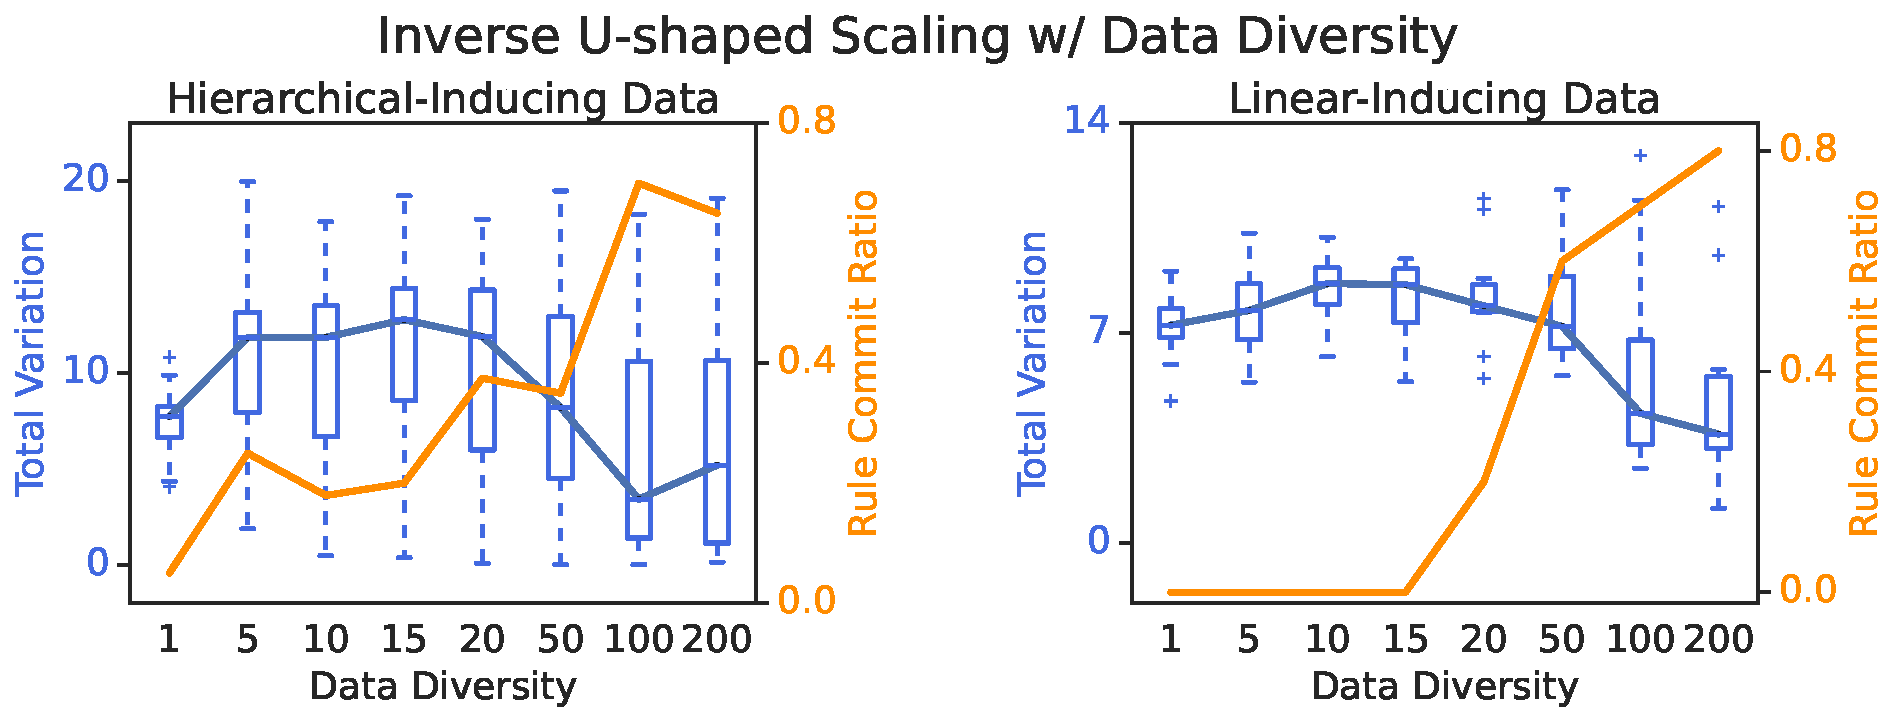
\includegraphics[width=0.8\linewidth]{figures/data_diversity_uscale.pdf}
    \caption{\textbf{Inverse U-shaped relationship between training stability and data diversity.} Whether training data favors the hierarchical (\textit{left}) or linear (\textit{right}) rule, diverse data promotes systematic rules over example memorization. At low diversity, training is stable but the model memorizes individual syntactic patterns rather than committing to a rule. With moderate data diversity, training becomes unstable. As diversity increases further, the model commits to a rule and training is the most stable.} 
    \label{fig:data_diversity_uscale}
    \vspace{-4px}
\end{figure}
\newpage
\section{Early investigations on visual quality in more complex environments}
\label{app:additonal_experiments}

In the main body of the paper, we evaluated the utility of \textsc{diamond} for the purpose of training RL agents in a world model on the well-established Atari 100k benchmark \citep{kaiser2019atari100k}, and demonstrated \textsc{diamond}'s diffusion world model could be applied to model a more complex 3D environment from the game \textit{Counter-Strike: Global Offensive}. In this section, we provide early experiments investigating the effectiveness of \textsc{diamond}'s diffusion world model by directly evaluating the visual quality of the trajectories they generate. The two environments we consider are presented in Section \ref{app:subsec:environments} below.

\subsection{Environments}
\label{app:subsec:environments}

\textbf{CS:GO.} 
We use the \textit{Counter-Strike: Global Offensive} dataset introduced by \citet{pearce2022counter}. Here we use the \textit{Clean} dataset containing 190k frames (3.3 hours) of high-skill human gameplay, captured on the \textit{Dust II} map. This contains observations and actions (mouse and keyboard) captured at 16Hz. We use 150k frames (2.6 hours) for training and 40k frames (0.7 hours) for evaluation. We resize observations to 64$\times$64 pixels, and use no augmentation.
%\footnote{\href{https://github.com/TeaPearce/Counter-Strike_Behavioural_Cloning}{\texttt{https://github.com/TeaPearce/Counter\-Strike\_Behavioural\_Cloning}}}.

\textbf{Motorway driving.} We use the dataset from \citet{santana2016learning}\footnote{\href{https://github.com/commaai/research}{\texttt{https://github.com/commaai/research}}}, which contains camera and metadata captured from human drivers on US motorways. We select only trajectories captured in daylight, and exclude the first and last 5 minutes of each trajectory (typically traveling to/from a motorway), leaving 4.4 hours of data. We use five trajectories for training (3.6 hours) and two for testing (0.8 hours). We downsample the dataset to 10Hz, resize observations to 64$\times$64, and for actions use the (normalized) steering angle and acceleration. During training, we apply data augmentation of shift \& scale, contrast, brightness, and saturation, and mirroring.

We note that the purpose of our investigation is to train and evaluate \textsc{diamond}'s diffusion model on these static datasets, and that we do not perform reinforcement learning, since there is no standard reinforcement learning protocol for these environments.


\subsection{Diffusion Model Architectures}

We consider two potential diffusion model architectures, summarized in Figure \ref{fig_architectures}.

\begin{figure}[h]
    \begin{center}
    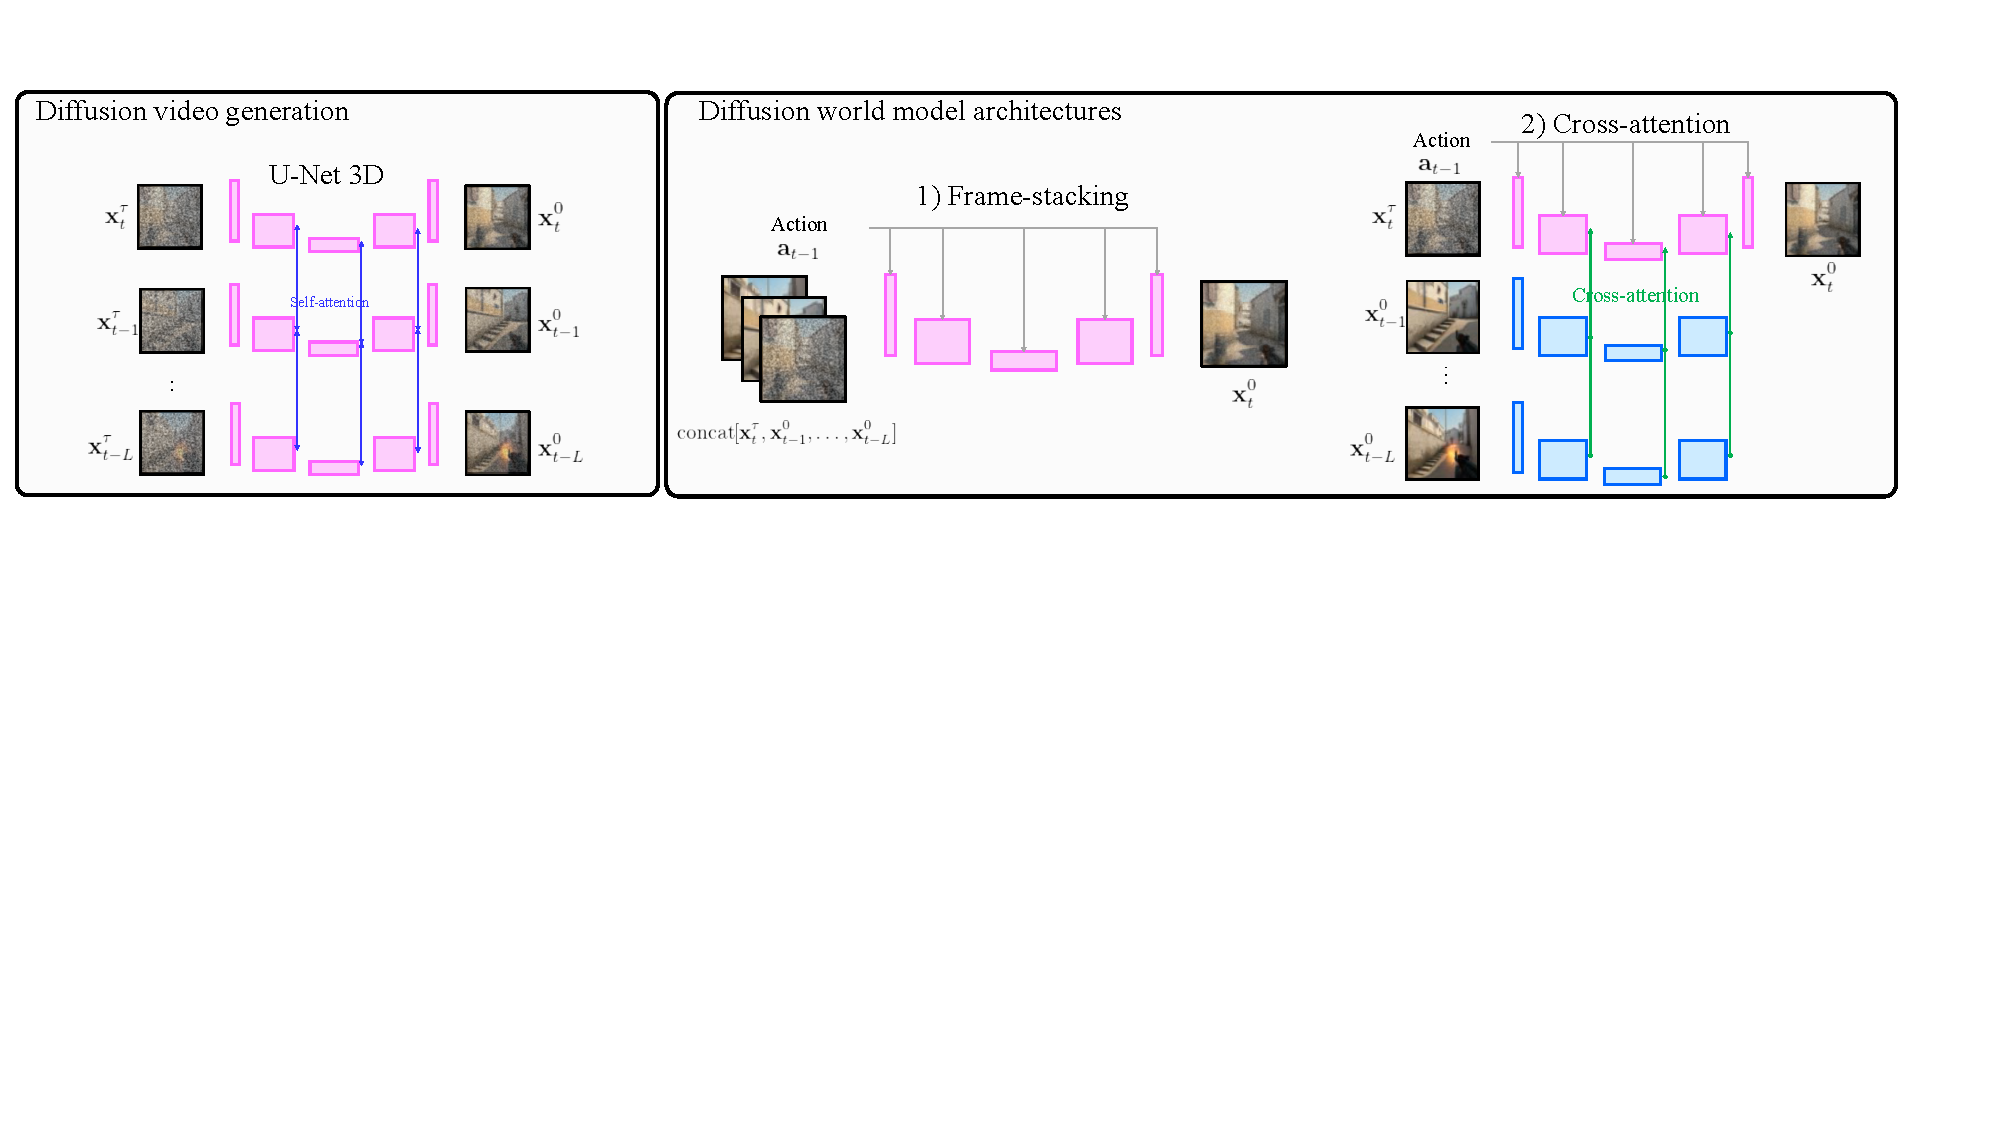
\includegraphics[width=0.99\columnwidth]{images/architectures_02.pdf}
    % \vskip -0.18in
    \caption{We tested two architectures for \textsc{diamond}'s diffusion model which condition on previous image observations in different ways. To illustrate differences with typical video generation models, we also visualize a U-Net 3D \citep{unet3d} which diffuses a block of frames simultaneously.}
    \label{fig_architectures}
    \end{center}
\end{figure}

\textbf{Frame-stacking.} The simplest way to condition on previous observations is by concatenating the previous $L$ frames together with the next noised frame, $\operatorname{concat}[ \x_t^{\tau}, \x_{t-1}^0, \dots, \x_{t-L}^0]$, which is compatible with a standard U-Net 2D \citep{ronneberger2015unet}.
This architecture is particularly attractive due to its lightweight construction, requiring minimal additional parameters and compute compared to typical image diffusion. This is the architecture we used for the main body of the paper.
% Experiments in Section \ref{sec_experiments} show this to be a surprisingly powerful mechanism for modeling both simple and complex environments. 

\textbf{Cross-attention.} 
The U-Net 3D \citep{unet3d}, also displayed for comparison in Figure \ref{fig_architectures}, is a leading architecture in video diffusion \citep{ho2022video}. We adapted this design to have an autoregressive cross-attention architecture, formed of a core U-Net 2D, that only receives a single noised frame as direct input, but which cross-attends to the activations of a separate history encoder network. This encoder is a lightweight version of the U-Net 2D architecture. Parameters are shared for all $L$ encoders, and each receives the relative environment timestep embedding as input.
The final design differs from the U-Net 3D which diffuses all frames jointly, shares parameters across networks, and uses self-, rather than cross-, attention.

\subsection{Metrics, Baselines and Compute}
\textbf{Metrics.}
To evaluate the visual quality of generated trajectories, we use the standard Fréchet Video Distance (\textbf{FVD}) \citep{unterthiner2018towards} as implemented by \citet{skorokhodov2022stylegan}. This is computed between 1024 real videos (taken from the test set), and 1024 generated videos, each 16 frames long (1-2 seconds). Models condition on $L=6$ previous real frames, and the real action sequence. On this same data, we also report the Fréchet Inception Distance (\textbf{FID}) \citep{heusel2017gans}, which measures the visual quality of individual observations, ignoring the temporal dimension. For these same sets of videos, we also compute the \textbf{LPIPS} loss \citep{zhang2018lpips} between each \textit{pair} of real/generated observations \citep{yan2023teco}.
\textbf{Sampling rate} describes the number of observations that can be generated, in sequence, by a single Nvidia RTX A6000 GPU, per second.

\textbf{Baselines.}
We compare against two well-established world model methods; DreamerV3 \citep{hafner2023dreamerv3} and \textsc{iris} \citep{iris2023}, adapting the original implementations to train on a static dataset. We ensured baselines used a similar number of parameters to \textsc{diamond}. Two variants of \textsc{iris} are reported; image observations are discretized into $K=16$ tokens (as used in the original work), or into $K=64$ tokens (achieved with one less down/up-sampling layer in the autoencoder, see Appendix E of \citet{iris2023}), which provide the potential for modeling higher-fidelity visuals. 
% The full list of hyperparameters is provided in the Appendix.
% IRIS: 35M for autoencoder, 88M for transformer, seq length 8...


\textbf{Compute.}
All models (baselines and \textsc{diamond}) were trained for 120k updates with a batch size of 64, on up to 4$\times$A6000 GPUs. Each training run took between 1-2 days.

\subsection{Analysis}

\begin{table}[h]
\caption{Results for 3D environments. These metrics compare observations from real trajectories and generated trajectories. The generated trajectories are conditioned on an initial set of $L=6$ observations and a real sequence of actions.}
\label{tab:video_results}
\begin{center}
\resizebox{0.999 \columnwidth}{!}{
\begin{tabular}{ l c c c c c c c c}
\toprule
\multicolumn{1}{c}{}  & \multicolumn{3}{c}{ ------------ \textbf{CS:GO} ------------} & \multicolumn{3}{c}{ ----------- \textbf{Driving} ----------- } & \multicolumn{1}{c}{\bf Sample rate} & \multicolumn{1}{c}{\bf Parameters} \\
\multicolumn{1}{l}{\bf Method}  & \multicolumn{1}{c}{\bf FID $\downarrow$} & \multicolumn{1}{c}{\bf FVD $\downarrow$ } & \multicolumn{1}{c}{\bf LPIPS $\downarrow$ } & \multicolumn{1}{c}{\bf FID $\downarrow$} & \multicolumn{1}{c}{\bf FVD $\downarrow$} & \multicolumn{1}{c}{\bf LPIPS $\downarrow$ }  & \multicolumn{1}{c}{\bf (Hz) $\uparrow$} & \multicolumn{1}{c}{\bf (\#)} \\ 
\hline \\
DreamerV3 & 106.8 & 509.1 & 0.173 & 167.5 & 733.7 & 0.160 & 266.7 & 181M \\
IRIS ($K=16$) & 24.5 & 110.1 & 0.129 & 51.4 & 368.7 & 0.188 & 4.2 & 123M \\
IRIS ($K=64$) & 22.8 & 85.7 & 0.116 & 44.3 & 276.9 & 0.148 & 1.5 & 111M \\
$\textsc{diamond}$ frame-stack (ours) & 9.6 & 34.8 & 0.107 & 16.7 & 80.3 & 0.058 & 7.4 & 122M \\
$\textsc{diamond}$ cross-attention (ours) & 11.6 & 81.4 & 0.125 & 35.2 & 299.9 & 0.119 & 2.5 & 184M \\
\bottomrule
\end{tabular}
}
\end{center}
\end{table}


Table \ref{tab:video_results} reports metrics on the visual quality of generated trajectories, along with sampling rates and number of parameters, for the frame-stack and cross-attention \textsc{diamond} architectures, compared to baseline methods. 
\textsc{diamond} outperforms the baselines across all visual quality metrics. 
This validates the results seen in the wider video generation literature, where diffusion models currently lead, as discussed in Section \ref{sec:related_work}.
The simpler frame-stacking architecture performs better than cross-attention, something surprising given the prevalence of cross-attention in the video generation literature. We believe the inductive bias provided by directly feeding in the input, frame-wise, may be well suited to autoregressive generation. Overall, these results indicate \textsc{diamond} frame-stack $>$ \textsc{diamond} cross-attention $\approx$ IRIS 64 $>$ IRIS 16 $>$ DreamerV3, which we found corresponds to our intuition from visual inspection.

In terms of sampling rate, \textsc{diamond} frame-stack (with 20 denoising steps) is faster than \textsc{iris} ($K=16$). \textsc{iris} suffers from a further 2.8$\times$ slow down for the $K=64$ version, verifying its sample time is bottlenecked by the number of tokens $K$.
On the other hand, DreamerV3 is an order of magnitude faster -- this derives from its independent, rather than joint, sampling procedure, and the flip-side of this is the low visual quality of its trajectories. 

\newpage


Figure \ref{fig_generation_egs} below shows selected examples of the trajectories produced by \textsc{diamond} in CS:GO and motorway driving.
% Trajectories produced by baselines are given in Appendix \tp{x}.
% , and comparisons with baselines in Appendix Figures \tp{x} \& \tp{y}.
The trajectories are plausible, often even at time horizons of reasonable length. In CS:GO, the model accurately generates the correct geometry of the level as it passes through the doorway into a new area of the map. In motorway driving, a car is plausibly imagined overtaking on the left.

\begin{figure}[h!]
    \begin{center}
    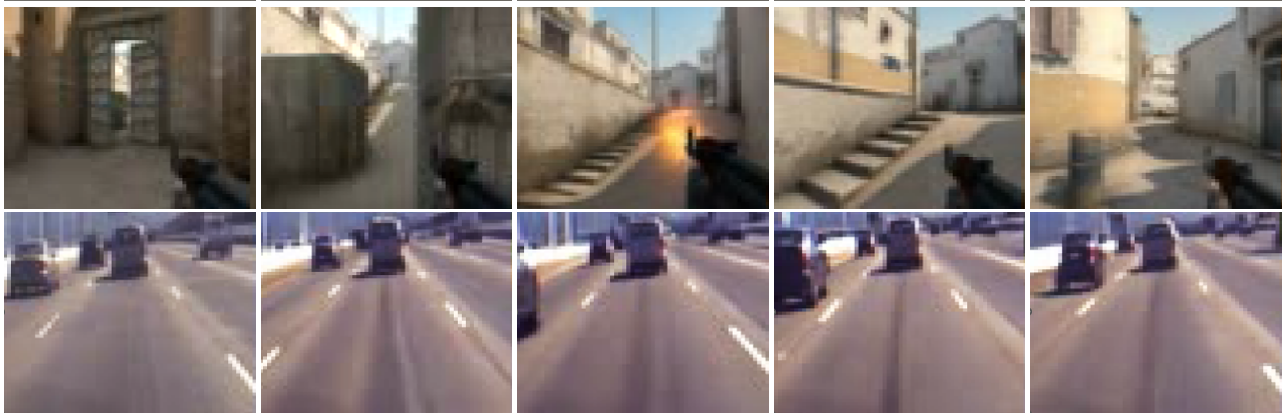
\includegraphics[width=0.8\columnwidth, height=0.4\columnwidth]{images/generation_egs_02.png}
    % \vskip -0.18in
    \caption{Example trajectories sampled every 25 timesteps from \textsc{diamond} (frame stack) for the modern 3D first-person shooter CS:GO (top row), and real-world motorway driving (bottom row).}
    \label{fig_generation_egs}
    \end{center}
\end{figure}


While the above experiments use real sequences of actions from the dataset, we also investigated how robust $\textsc{diamond}$ (frame stack) was to novel, user-input actions.
Figure \ref{fig_driving_action} shows the effect of the actions in motorway driving -- conditioned on the same $L=6$ real frames, we generate trajectories conditioned on five different action sequences. In general the effects are as intended, e.g. steer straight/left/right moves the camera as expected.
Interestingly, when `slow down' is input, the distance to the car in front decreases since the model predicts that the traffic ahead has come to a standstill.
%This is an interesting causal confusion, since from the action alone, slowing down should in principle \textit{increase} the distance to the car in front. 
Figure \ref{fig_csgo_action} shows similar sequences for CS:GO. For the common actions (mouse movements and fire), the effects are as expected, though they are unstable beyond a few frames, since such a sequence of actions is unlikely to have been seen in the demonstration dataset.
% We found that $\textsc{wm}$ had not learned to model the impact of less common actions such as `jump'.
We note that these issues -- the causal confusion and instabilities -- are a symptom of training world models on offline data, rather than being an inherent weakness of $\textsc{diamond}$.
% Also acknowledge the offdistribution problem, but more a problem of data than model.


\begin{figure}[h!]
    \begin{center}
    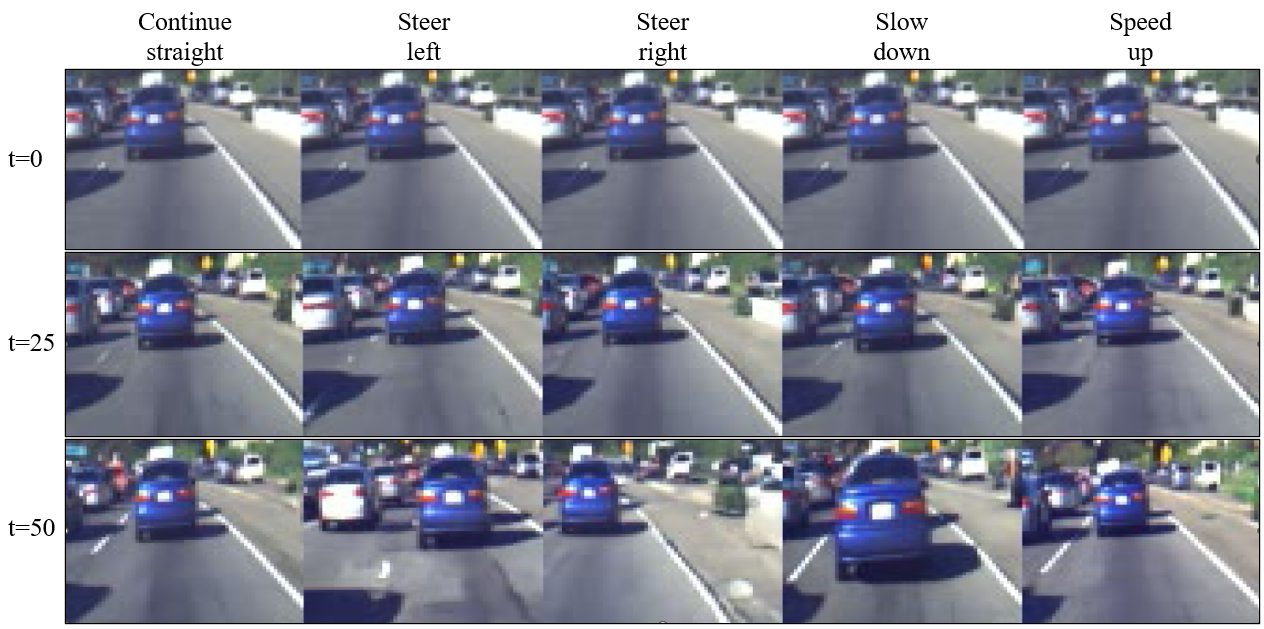
\includegraphics[width=0.99\columnwidth]{images/driving_action_02.png}
    % \vskip -0.18in
    \caption{Effect of fixed actions on sampled trajectories in motorway driving. Conditioned on the same initial observations, we rollout the model applying differing actions. Interestingly, the model has learnt to associate 'Slow down' and 'Speed up' actions to the whole traffic slowing down and speeding up.}
    \label{fig_driving_action}
    \end{center}
\end{figure}


\begin{figure}[t!]
    \begin{center}
    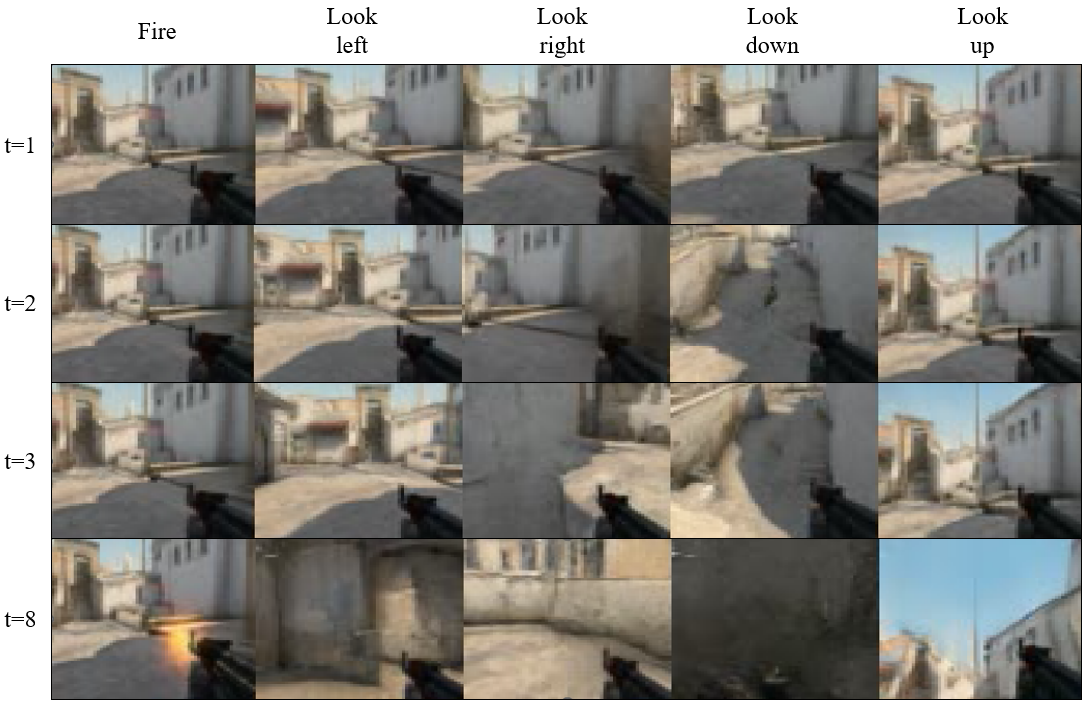
\includegraphics[width=0.9\columnwidth]{images/csgo_action_01.png}
    % \vskip -0.18in
    \caption{Effect of fixed actions on sampled trajectories in CS:GO. Conditioned on the same initial observation, we rollout the model applying differing actions. Whilst in immediate frames these have the intended effect, for longer roll-outs the observations can degenerate. For instance, it would have been very unlikely for the human demonstrator to look directly into ground in this game state, so the world model is unable to generate a plausible trajectory here, and instead snaps onto another area of the map when looking down does make sense.}
    \label{fig_csgo_action}
    \end{center}
\end{figure}
\clearpage


%%%%%%%%%%%%%%%%%%%%%%%%%%%%%%%%%%%%%%%%%%%%%%%%%%%%%%%%%%%%

\end{document}
